%_*_Mode: LaTeX_*_
\documentclass[a4paper]{article}
%%%% Az ábrákhoz szükséges csomagok
\usepackage{graphicx}

%%%% A magyar nyelvvel és a karakterek kódolásával
%%%% kapcsolatos csomagok
\usepackage[T1]{fontenc}
\usepackage{t1enc}
\usepackage[utf8x]{inputenc}
\usepackage[magyar]{babel}
\usepackage{indentfirst}  % Az első bekezdést is behúzza.
\frenchspacing   % A mondatvégek után azonos szóköz van, mint máshol
    % (Az angolban nagyobb a szokás. Ez az alapbeállítás.)

% A pdf kisebb és olvashatóbb lesz, ha times betűket használok.
\usepackage{times}
\usepackage{tikz}
\usepackage{array} %tabularban math mód
\usetikzlibrary{arrows}
\tikzset{ %inner sep = 0.5mm,
  %minimum size = 5mm,
  {selected path/.style} ={draw,opacity=.5,line width=3pt,green},
  {hide path/.style} ={selected path,white,opacity=.9},
  {base point/.style} ={circle,draw=blue!60,fill=blue!30,inner sep=0},
  {small point/.style} ={base point, minimum size= 1mm},
  {middle point/.style} ={base point, minimum size= 3mm},
  {large point/.style} ={base point, minimum size= 10mm},
  {future point/.style} ={circle,color=white,draw},
  point/.style ={circle,draw=black!60,fill=black!20},
  {new point/.style} ={point,fill=blue!30,draw=blue!60},
  {edge/.style} ={thick,draw},
  {new edge/.style} ={draw,thick,-, blue!50},
  {box/.style}={rectangle,  minimum height=1cm,
                anchor=south west, draw, rectangle,
                fill=yellow!20,text centered, text width= 4cm},
  >=latex,
  state/.style = {thick, circle, draw, color = black,
                  fill = red!20, minimum size = 6mm},
  finalstate/.style = {state, fill=green!20, double},
  automat/.style = {thick, draw, color = black, fill = #1!12,
                  minimum size = 10mm},
  automat/.default = black,
  point/.style ={circle,draw=blue!60,fill=blue!30,
                  inner sep=0, minimum size= 1mm},
 }

\usepackage{mathptm}  % A mathptm a képletekben is times-t használ.
    % Összeakad az amssymbol vagy az amsmath csomaggal (amsfont).
    % Talán nincsenek telepítve valamilyen fontjaim.

%%%%%%%%%%%%%%%%%%%%%%%%%%%%%%%%%%%%%%%%%%%%
%%%% Az Amerikai Matematikai Társulat (AMS)
%%%% hasznos csomagja  (pl. \dfrac)
\usepackage{amsmath}

% Magyar függvénynevek
\DeclareMathOperator{\tg}{tg}
\DeclareMathOperator{\sh}{sh}
\DeclareMathOperator{\ch}{ch}
\DeclareMathOperator{\cth}{cth}
\DeclareMathOperator{\ctg}{ctg}
\DeclareMathOperator{\arctg}{arctg}
\DeclareMathOperator{\arcctg}{arcctg}
\DeclareMathOperator{\arsh}{arsh}
\DeclareMathOperator{\arch}{arch}
\DeclareMathOperator{\arth}{arth}
\DeclareMathOperator{\arcth}{arcth}

% Ezzel a duplaszárú betűk elérhetőek.
% Pl. valós számok halmazjele:  \mathbb{R}
% (Nem tökéletes, mert mindkét oldalon dupla.)
\usepackage{amssymb}

% \usepackage{t1enc}
% \usepackage[T1]{fontenc}      %ujabb betuertelmezo
% \usepackage[latin2]{inputenc}
% \usepackage{graphicx}
\usepackage[magyar]{babel}
% \usepackage{pslatex}
\usepackage{indentfirst}
% \frenchspacing 
\usepackage{pxfonts} %mathbb
\usepackage{html}
\newcommand{\name}{\textsc}
\newcommand{\segitseg}{\textbf{Segítség:}\:}
\newcommand{\megoldas}{\textbf{Megoldás:}\:}
\usepackage{framed} %leftbar
\usepackage[a4paper,margin=1cm,footskip=.5cm]{geometry}

%\newenvironment{feladat}{{\bfseries Feladat:}\:}{}
%\newenvironment{pelda}{{\bfseries Példa:}\:\par}{}
\newtheorem{feladat}{feladat}[section]
\newtheorem{pelda}{példa}[section]
\newtheorem{definicio}{definíció}[section]
\newtheorem{tetel}{tétel}[section]

\newcommand{\spacer}[1][2 cm]{\rule{#1}{.4pt}\rule{0pt}{2em} }

%TODO feladatok, bevezető, Feynman-gráf kép, konstansok

\tikzset{
  >=latex,
  state/.style = {thick, circle, draw, color = black, fill =
red!20, minimum size = 6mm},
  finalstate/.style = {state, fill=green!20, double},
  automat/.style = {thick, draw, color = black, fill = #1!12, minimum
  size = 10mm},
  automat/.default = black,
  point/.style ={circle,draw=blue!60,fill=blue!30,inner sep=0, minimum
size= 1mm}
}

\begin{document}

\title{Formális nyelvek és automaták}
\author{Horváth Árpád}
\maketitle

Nézzük először vázlatosan a félév fontosabb fogalmait!

{Nyelvek, nyelvtanok és automaták kapcsolata általában}

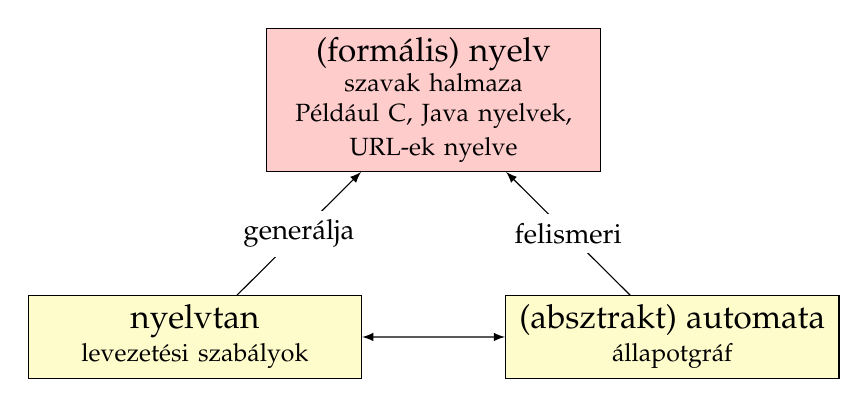
\begin{tikzpicture}[>=latex,yscale=1.5]
    \node[box,fill=red!20] (nyelv) at (0,0) {\large (formális) nyelv\\
    \small szavak halmaza\\
    Például C, Java nyelvek,\\
    URL-ek nyelve
    };
    \node[box] (nyelvtan) at (210:3.5) { 
    \large nyelvtan\\ \small levezetési szabályok};
    \node[box] (automata) at (330:3.5) {\large (absztrakt) automata\\ \small állapotgráf};
    \draw[->] (nyelvtan) edge node[fill=white] {generálja} (nyelv);
    \draw[->] (automata) edge node[fill=white] {felismeri} (nyelv);
    \draw[<->] (automata) -- (nyelvtan);
\end{tikzpicture}

Ezeket a nyelveket majd osztályokba fogjuk sorolni. Például a
környezetfüggetlen nyelvekhez tartoznak a programozási nyelvek.

{Környezetfüggetlen nyelvek, környezetfüggetlen nyelvtanok ill.
veremautomaták kapcsolata} 

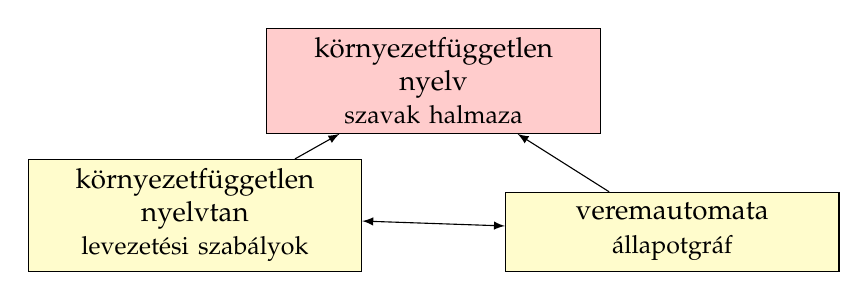
\begin{tikzpicture}[>=latex]
    \node[box,fill=red!20] (nyelv) at (0,0) {környezetfüggetlen nyelv\\
    \small szavak halmaza};
    \node[box] (nyelvtan) at (210:3.5) {környezetfüggetlen 
    nyelvtan\\ \small levezetési szabályok};
    \node[box] (automata) at (330:3.5) {veremautomata\\ \small állapotgráf};
    \draw[->] (nyelvtan) -- (nyelv);
    \draw[->] (automata) -- (nyelv);
    \draw[<->] (automata) -- (nyelvtan);
\end{tikzpicture}

A környezetfüggetlen nyelvekhez hasonló diagram rajzolható fel a
környezetérzékeny és az általános nyelvtanok esetén is, csak az automata
típusa lesz más és más. Sőt a reguláris nyelvtanok esetén is, de ott a
nyelvnek még egy hasznos megadási módot fogunk tanulni: az úgynevezett
reguláris kifejezésre illeszkedő szavak is reguláris nyelvet alkotnak.

{Reguláris nyelvek, kifejezések és nyelvtanok ill. véges automaták
kapcsolata}

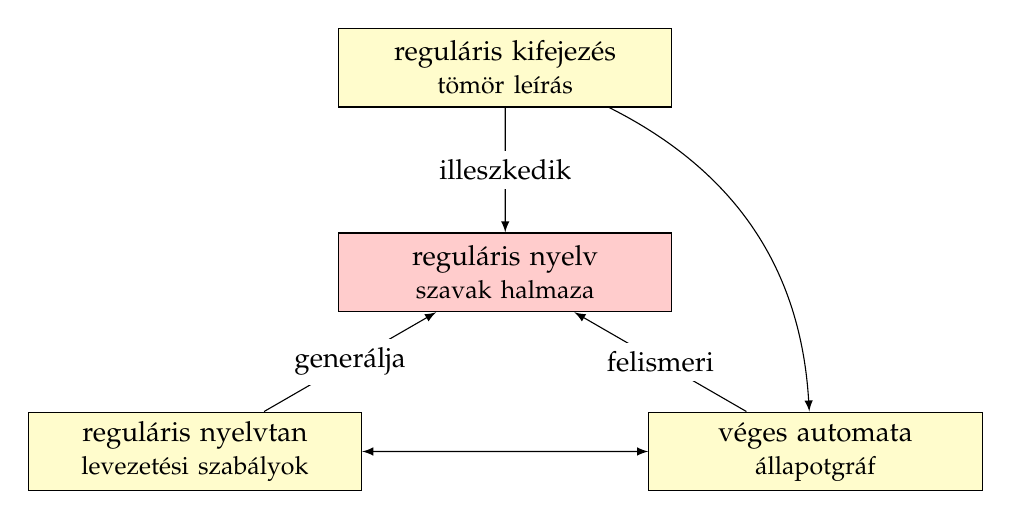
\begin{tikzpicture}[>=latex,scale=1.3]
    \node[box,fill=red!20] (nyelv) at (0,0) {reguláris nyelv\\
    \small szavak halmaza};
    \node[box] (kif) at (0,2) {reguláris kifejezés\\ \small tömör leírás};
    \node[box] (nyelvtan) at (210:3.5) {reguláris
    nyelvtan\\ \small levezetési szabályok};
    \node[box] (automata) at (330:3.5) {véges automata\\ \small állapotgráf};
    \draw[->] (kif) edge node[fill=white] {illeszkedik} (nyelv);
    \draw[->] (nyelvtan) edge node[fill=white] {generálja} (nyelv);
    \draw[->] (automata) edge node[fill=white] {felismeri} (nyelv);
    \draw[<->] (automata) -- (nyelvtan);
    \draw[->] (kif) edge [bend left] (automata);
\end{tikzpicture}

\newpage

%\newpage % ++ +++ ++  ++ +++ ++  ++ +++ ++  ++ +++ ++  ++ +++ ++
\section{Formális nyelvek}

Ebben a segédletben néha használom a \emph{szó} kifejezést, mely a
Bach-könyvben \emph{mondatként}* szerepel.

Pár azonos értelemben használt kifejezés a szakirodalomból:

ábécé = alfabeta* (veremábécé = verem alfabetája*)

nyelvtan*=grammatika* de nyelvtan$\neq$nyelv!

DFA = FDA = determinisztikus véges automata*

reguláris kifejezés = reguláris halmaz*

végállapot = elfogadó állapot*

A *-gal jelölteket használja a könyv.

De kezdjük az elején.

\subsection*{Formális nyelvek alapfogalmai és jelölései}
\begin{definicio} A formális nyelvek alapvető definíciói.
\par
\begin{itemize}
\item Ábécé: szimbólumok véges halmaza ($\Sigma$) Ezek egyesítése,
különbsége a halmazokéhoz hasonlóan definiált.
\item Ábécé betűi: a szimbólumok ($a$, $b$, $c_k$)\: $a\in \Sigma$
\item Szó: szimbólumok véges sorozata
(A szavakat később gyakran az ábécé végéről vett jelekkel fogjuk
jelölni ($v, w, x, y, z$), ebben az esetben azt fogja jelenteni, hogy csak terminális
szimbólumok vannak benne; hasonló nagybetűkkel ($V, W, X, Y, Z$) pedig
olyanokat, amelyben csak nemterminálisok; görög betűkkel  ($\alpha$,
$\beta$, $\omega$) pedig olyanokat, amelyikben bármelyik.)
\item Szó hossza: a sorozat hossza ($len(\alpha)$) (Az angol
length=hossz szóból.) 
\item Üres szó ($\varepsilon$): melyre $len(\varepsilon) = 0$ (Ha a
szavakra úgy gondolunk, mint a programozási nyelvek sztringjeire, akkor
a $\varepsilon$ az üres sztringnek, felel meg. Az $\varepsilon$ talán
könnyebben megjegyezhető úgy, hogy az az angol empty szó kezdőbetűjének
görög megfelelője (kis epszilon).)
\item Szavak konkatenációja (összefűzése):\\ $y w = a_1 a_2 a_3 \cdots a_n
	b_1 b_2 \cdots b_m$,
	ahol  $y =a_1 a_2 a_3 \cdots a_n$, $w = b_1 b_2 \cdots b_m$
	(Asszociatív, kommutatív, egységelemes-e? $len(y w)=?$)
\item Tükörkép: $y^{-1}=a_n \cdots a_2 a_1$ a fenti ipszilonnal, azaz a
betűit fordított sorrendben írom le.
\item Hatvány: $y^0=\varepsilon, y^1=y,
	y^n=y^{n-1}y$. (Pl. $(ab)^3=ababab$)
\item $\Sigma^*$ a $\Sigma$ ábécéből alkotott összes szó, beleértve az
    üres szót is.\\
    Például $\{a,b\}^*=\{\varepsilon, a, b, aa, ab, ba, bb, aaa, \ldots
    abbaaab, \ldots\}$
\item $\Sigma$ ábécéből alkotott formális nyelv (${\cal L}(\Sigma)$ vagy ${\cal L}$):
	bármely ${\cal L}(\Sigma) \subseteq \Sigma^*$
\end{itemize}
\end{definicio}

\begin{pelda}
  Példák nyelvekre.
\begin{itemize}
\item $\Sigma=\{0, 1\}$,\\ ${\cal L}_0(\Sigma) = \emptyset$,
	${\cal L}_e(\Sigma) = \{\varepsilon \}$,
	${\cal L}_1(\Sigma) = \{01, 0, \varepsilon \}$,
	${\cal L}_2(\Sigma) = \{y0y^{-1} \mid y\in \{0; 1\}^*\}$,   
\item $\Sigma' = \{ if; then; a; b; c\} \quad {\cal L}_1(\Sigma')=\{\mbox{c; if a then b; if a then
if b then c}\}$
\item $01'01010 \in {\cal L}_1(\Sigma){\cal L}_2(\Sigma)$ \quad az ' csak a határt jelöli
\end{itemize}
\end{pelda}

Nyelvtanok megadásához 4 dolgot kell megadni: $G(\Sigma; N; S; P)$\\
$\Sigma$: terminális szimbólumok, $N$: nemterminális szimbólumok, $S$: kezdőszimbólum, $P$: helyettesítési szabályok.
Általában a jelölésrendszer egyértelműsége miatt a $P$ helyettesítési
szabályok megadása elegendő. Általában ugyanis a nemterminálisokat
nagybetűvel jelöljük, ezek közül a kezdőszimbólumot S-el, a többi
szimbólum terminális szimbólum.

A programozási nyelvek környezetfüggetlen nyelvtanának leírásában
általában nyíl helyett \verb|::=| jelölést használjuk, és gyakran a
terminálisokat idézőjelbe rakják. Erről az úgynevezett Backus--Naur
jelölésről a segédletben később esik szó.

\begin{pelda}
\label{pl:c}
Határozzunk meg az alábbi helyettesítési szabályok esetén mik lesznek a
nem terminális és terminális szimbólumok!  Vezessünk le az
értékadó\_kifejezés szimbólumból egy szót!

{\it
\begin{enumerate}
\item értékadó\_kifejezés ::= változó értékadó\_operátor értékadó\_kifejezés
\item értékadó\_kifejezés ::= változó
\item értékadó\_operátor ::=  \verb|"="| 
\item értékadó\_operátor ::=  \verb|"*="|
\item értékadó\_operátor ::=  \verb|"/="|
\item értékadó\_operátor ::=  \verb|"+="|
\item értékadó\_operátor ::=  \verb|"-="|
\item változó ::= \verb|"a"|
\item változó ::= \verb|"b"|
\end{enumerate}
}

(A Kernighan--Ritchie: \emph{A C programozási nyelv} (1996) című könyv
258. oldalán található \emph{A C nyelv szintaktikájának összefoglalása}.
Egy részének jelentősen egyszerűsített változata szerepel itt.)

A helyettesítési szabályok első sorának jobboldalán három tag szerepel,
mindhárom nemterminális, a második sor jobb oldalán egy nemterminális, a
következő sorok jobb oldalán terminális szimbólumok szerepelnek. A
nemterminális szimbólumok:\\
$N=\{$értékadó\_kifejezés, változó, értékadó\_operátor$\}$\\
A terminális szimbólumok: $\Sigma=\{$a, b, =, *=, /=, +=, -=$\}$\\

Kiindulva az {\it értékadó\_kifejezés} nemterminális szimbólumból, az
alábbi lépésekben megkaphatunk egy csupán terminális szimbólumból álló
kifejezést:

{\it
\noindent
értékadó\_kifejezés   \quad$\Rightarrow$ (1)\\
változó értékadó\_operátor értékadó\_kifejezés   \quad$\Rightarrow$ (3)\\
változó = értékadó\_kifejezés   \quad$\Rightarrow$ (8)\\
a = értékadó\_kifejezés   \quad$\Rightarrow$ (1)\\
a = változó értékadó\_operátor értékadó\_kifejezés   \quad$\Rightarrow$
(4)\\
a = változó *= értékadó\_kifejezés   \quad$\Rightarrow$ (9)\\
a = b *= értékadó\_kifejezés   \quad$\Rightarrow$ (8)\\
a = b *= a\\
}

{\small
(Ez a kifejezés amúgy C-ben érvényes kifejezés, először a *= kifejezés
hajtódik végre, megszorozva a b értékét a-val, ez kerül először b-be,
majd ez az eredmény kerül a-ba is.)
}
\end{pelda}

A terminális és nemterminális szimbólumok (pl. változó) egy ábécét
alkotnak a korábbi elnevezéseink szerint, a kapott kifejezés pedig egy
terminális szimbólumokból álló szó.

Az $P$-ben található helyettesítési szabályok segítségével az $S$
kezdőszimbólumból kiindulva egy vagy több lépésben levezethetünk
bizonyos szavakat, amelyek csak nemterminális szimbólumokból állnak. Az
így levezethető szavakat nevezzük a $G$ nyelvtan által generált
nyelvnek.  Jele: ${\cal L}(G)$.

A továbbiakban azt vizsgáljuk, hogy milyen lehetőségeink vannak annak
ellenőrzésére, hogy egy szó benne van-e a nyelvtan által generált
nyelvben.

A feladatmegoldás során a \emph{problémát az általános megoldása felől
közelítjük} meg ahelyett, hogy elköteleznénk magunkat a technikai
részletek mellett, hogy például a feladatot hardveresen vagy szoftverrel
oldjuk-e meg.

A nyelv szavait felismerő elméleti konstrukciókat \emph{automatáknak}
fogjuk nevezni. Ezeknek több típusa van, és hogy melyik az a
legegyszerűbb típus, amit alkalmazni tudunk, a nyelv típusától függ.
Vizsgáljuk meg tehát, milyen típusok vannak.

Az \ref{pl:c}.  példában láttunk egy példát egy C-szerű nyelv egy
részletének leírásából.  Ott a nemterminális szimbólumok esetén olyan
leírásokat találhatunk, mint  a változó, értékadó\_kifejezés, vagy
értékadó\_operátor. A továbbiakban mi általában ezeknél rövidebb
jelölésmódot fogunk alkalmazni. Latin nagybetűkkel ($S,\:A,\:B$) fogjuk
jelölni a nemterminális szimbólumokat, és kisbetűvel (a, b, c) a
terminális szimbólumokat.

\subsection*{Nyelvtanok és nyelvek típusai (Chomsky-hierarchia)}

A nyelvek típusait a nyelvtanok típusaiból fogjuk származtatni. Először
tehát ezt vizsgáljuk meg.  Először egy táblázatban összefoglalom a
nyelvtanok típusait, majd részletesebben kifejtem.

Legyen $\alpha, \beta, \omega \in (\Sigma \cup N)^* \quad A, B \in N
\quad a \in \Sigma$

\begin{tabular}{|lll|}
\hline
szabályok típusa & nyelvtan típusa&automata\\
\hline
$\alpha A \beta \to \omega$ & 0-típusú, általános&Turing-gép\\
$\alpha A \beta \to \alpha\omega\beta$ & 1-típusú, környezetérzékeny&\\
$A \to \omega$ & 2-típusú, környezetfüggetlen (CF)&PDA\\
$A \to aB$ vagy $A \to a$ & 3-típusú, reguláris&DFA\\
\hline
\end{tabular}

A környezetfüggetlen nyelvnél nem szoktuk megengedni, hogy a jobboldalt
üres szó szerepeljen. Így a környzetfüggetlen nyelv nemnövelő lesz, ami
azt jelenti, hogy a levezetés egyik lépésében sem csökken a szimbólumok
száma.

Megengedjük viszont az $S\to \varepsilon$ szabályt a környzetfüggetlen
nyelv és a reguláris nyelvek esetén, ha sehol sem szerepel a $\to$
jobboldalán $S$. Ha ezt hozzávesszük, akkor egy nyelv típusa nem fog
függeni attól, ha az üres szót $\varepsilon$ hozzáadjuk, vagy elvesszük
belőle. (A Python programozási nyelvben például egy 0 bájtos fájl
érvényes program, csak nem csinál semmit.)

Az általános nyelvtan tényleg a legáltalánosabb. A
szabályoktól csak azt követeljük meg, hogy a baloldalán legyen nem
terminális szimbólum, és egy ilyen részt bármilyen szóvá átalakíthatunk.

A környezetérzékeny (Context Sensitive, CS) nyelvtannál már
megköveteljük, hogy ha a szabály bal oldalán ha a nemterminális
szimbólum mellett annak jobb és baloldalán valamilyen szó áll, akkor az
változatlanul maradjon meg az átalakított szó elején.

A környezetfüggetlen (Context Free, CF) nyelvtannál már csak
egy nemterminális szimbólumot alakíthatunk át tetszőleges szóvá. A
környezetfüggetlen tényleg részhalmaza az előzőnek.  A
környezetérzékenyből csak azokat a speciális átalakítási szabályokat
engedjük itt meg, ahol $\alpha=\beta=\varepsilon$, azaz mindkettő üres
szó.

\begin{definicio}
A nyelvet n-típusúnak nevezünk, ha van olyan n-típusú
nyelvtan, amely a nyelvet generálja. (Pl: környezetfüggő nyelvet generál
a környezetfüggő nyelvtan.)
\end{definicio}

Eszerint például a környezetfüggetlen, nyelvtanok által generált
nyelveket környezetfüggetlen nyelveknek nevezzük. Ezekhez a nyelvekhez
tartozik sok programozási nyelv.

A reguláris nyelvtanok csak egész speciális formájú átalakításokat
engednek meg, ahogy a táblázatban látjuk, egy nemterminális szimbólumot
alakíthatunk egy terminálissá vagy egy terminális utáni nemterminálissá.

A környezetfüggetlen nyelv szoros kapcsolatban van a programozási
nyelvek nagy részében alapból vagy függvénykönyvtárak segítségével
elérhető reguláris kifejezésekkel.

\section{Véges automaták, mint nyelvek felismerői}

A véges automaták, az alábbi ábrán látható módon, egy szalagból,
és egy véges vezérlőműből áll. A szalagon található egy szó, amely egy
adott ábécé szimbólumaiból áll. A véges vezérlőmű minden lépésben
beolvas egy szimbólumot, és a mozgási szabályok figyelembevételével új
állapotba kerülhet. Előfordulhat, hogy az adott állapot esetén adott
szalagábécébeli szimbólum esetén nincs szabály arra, milyen állapotba
kerüljön. Ilyenkor a felismerés elakad.

A szó felismerésére először azt az egyszerűbb változatot vizsgáljuk meg,
amikor minden állapotban minden szalagábécébeli szimbólum esetén
egyetlen mozgási szabály van. Ilyenkor azt mondjuk, hogy a véges
automata determinisztikus. 
Determinisztikus véges automata (DFA) esetén akkor mondjuk, hogy egy
szalagon szereplő szót felismert, ha a szót végig tudta olvasni, és a
végigolvasás végén végállapotba került.

Elvileg megállapítható azoknak a szavaknak a (véges vagy végtelen)
halmaza, amelyet az automata felismer. Az ilyen szavak halmaza nyelvet
alkot. Ezt a nyelvet nevezzük az automata által felismert nyelvnek. A
véges automaták esetén be fogjuk látni, hogy a véges automaták által
felismert nyelv csak reguláris nyelv lehet, és bármely reguláris nyelv
esetén van olyan véges automata, amely az adott nyelvet ismeri fel.

A véges automata szalagábécéje lesz a felismert nyelv ábécéje, ezért
jelöljük $\Sigma$-val mindkettőt.

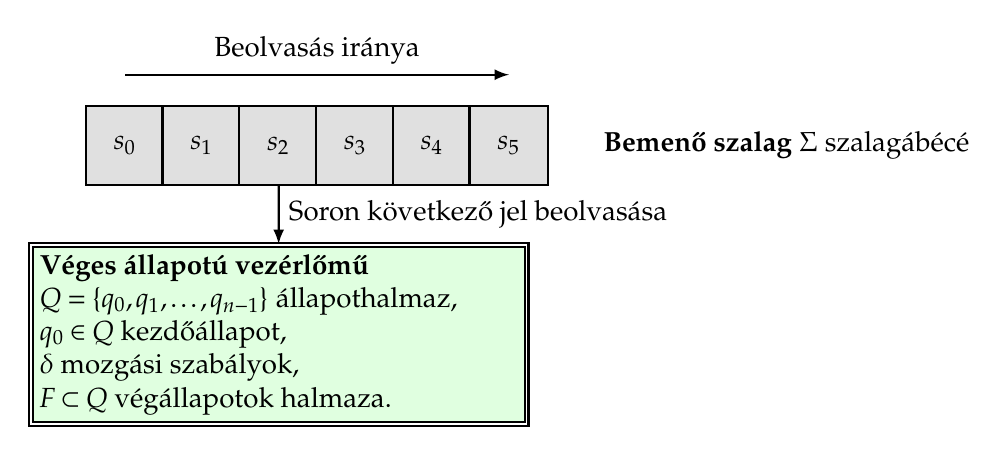
\begin{tikzpicture}[scale=1.5]
\node[automat] (s0) at (0,0) {$s_0$};
\node[automat] (s1) at (0.65,0) {$s_1$};
\node[automat] (s2) at (1.3,0) {$s_2$};
\node[automat] (s3) at (1.95,0) {$s_3$};
\node[automat] (s4) at (2.6,0) {$s_4$};
\node[automat] (s5) at (3.25,0) {$s_5$};
\node (S) at (5.6,0) {\textbf{Bemenő szalag} $\Sigma$ szalagábécé};
\node[automat=green, double] (VA) at (1.3,-1.6)
{\begin{minipage}{.5\textwidth}
    \textbf{Véges állapotú vezérlőmű}\\
    $Q = \{q_0, q_1, \dots, q_{n-1}\}$ állapothalmaz,\\
    $q_0 \in Q$ kezdőállapot,\\
    $\delta$ mozgási szabályok,\\
    $F\subset Q$ végállapotok halmaza.
\end{minipage}};
\path[thick, ->] (s2) edge node[right] {Soron következő jel beolvasása} (VA);
\path[thick, ->] (0,0.6) edge node[above] {Beolvasás iránya} (3.25,0.6);
\end{tikzpicture}

Egy véges automata vezérlőművét legszemléletesebben állapotgráffal
adhatjuk meg, ami egy irányított gráf: nyíl mutat a kezdeti (általában
$q_0$-lal vagy $S$-el jelölt) állapotra. A nyilakon szereplő szimbólumok
(a $\Sigma$ szalagábécéből) jelzik, hogy egy adott állapotból azt olvasván a
szalagról hova jut tovább. A kettős körök jelzik a végállapotokat. 

A véges automatákat mi állapotgráffal fogjuk ábrázolni általában. Tudni
kell azonban, hogy minden állapotgráfhoz 5 dolgot kell tudni, amiknek a
jelei $(Q, \Sigma, \delta, q_0, F)$. $Q$ az automata állapotainak a
halmaza, $\Sigma$ a felismerendő nyelv ábécéje, $\delta$ függvény a
mozgási szabályokat tartalmazza, egy-egy $q_i$ állapotra és ábécébeli
$a$ szóra $\delta(q_i, a_j)$ visszaadja, hogy milyen következő állapotba
kerül az automata. Tudnunk kell, hogy melyik állapot a kezdőállapot, de
ez a jelöléséből ($q_0$ vagy $S$) is nyilvánvaló szokott lenni
(Állapotgráfon egy rövid nyilacska az állapothoz). És végül tudnunk
kell, melyek a végállapotok ($F$: végállapotok halmaza; állapotgráfon
dupla karika jelöli).  Gyakran az egész automatának nevet is szoktunk
adni (pl. $M, M_1, M_2, M'$), ilyenkor az alábbi jelölést használjuk
$M(Q, \Sigma, \delta, q_0, F)$: 

\emph{Nemdeterminisztikus a véges automata} (NFA), ha van olyan állapot,
amelyből egy terminális szimbólum hatására legalább kétfelé mehetünk
tovább.  NFA esetén akkor mondjuk, hogy egy szót az automata felismer,
ha (az általában több lehetséges útvonal közül) van olyan
állapotsorozat, amelynek során végig tudjuk olvasni a szót, és
végállapotba jutunk.

Tudni kell:
\begin{itemize}
\item megállapítani, hogy egy szót felismer-e egy DFA, NFA,
\item egy mozgássorozatot konfigurációsorozattal leírni,
\item egyszerűbb automatákból megállapítani, milyen nyelvet ismer fel,
és azt halmazjelölésekkel felírni,
\item megállapítani, hogy egy véges automata DFA vagy NFA-e,
\item hogyan alakíthatjuk át a nemdeterminisztikus automatákat
determinisztikussá.
\end{itemize}

Bach 2.2. szakasz, Determinisztikus és nemdeterminisztikus véges
automaták. A 37. oldalon van egy NFA$\rightarrow$DFA átalakítás, én
ennél egyszerűbbeket kérdezek, de azt érdemes végigolvasni és megérteni.
 
\section{Reguláris nyelvek és véges automaták}

Az automaták és a nyelvek között a táblázatban látható kapcsolat van.
Bármely véges automata által felismert összes szóból alkothatunk egy
nyelvet, és ez mindig reguláris nyelv lesz. Fordítva: minden reguláris
nyelvhez hozhatunk létre olyan véges automatát, amely azt a nyelvet
ismeri fel. Hasonló a kapcsolat a többi, a táblázatban feltüntetett
automata és nyelvcsalád között. A véges automata helyett azért írtunk
DFA-t, mert belátható, hogy minden véges automata átalakítható
\emph{determinisztikus} véges automatává, úgy, hogy ugyanazokat a
szavakat ismerje fel illetve utasítsa el mint az eredeti. Tehát a
determinisztikus véges automaták mindarra képesek, mintha még hozzájuk
vennénk a nem determinisztikusakat (NFA-kat) is.

Az alábbiakban megadjuk, hogyan lehet átalakítani egy reguláris
nyelvtant véges automatává úgy, hogy a véges automata ugyanazt a nyelvet
ismerje fel, mintha amit a reguláris nyelvtan generál. Mivel ez az
átalakítás mindig lehetséges, ebből következik, hogy a reguláris
nyelvekhez mindig tartozik azt felismerő véges automata.

\noindent
\frame{
\begin{minipage}{.98\textwidth}
\textbf{Reguláris nyelvtan $\rightarrow$ véges automata átalakítási
szabályok}

Kell kezdetben egy kezdőállapot 
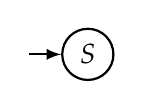
\begin{tikzpicture}[scale=1.5]
\node[state,fill=white] (S) at (0,0) {$S$} edge[<-,thick] (-.5,0);
\end{tikzpicture},

és egy végállapot
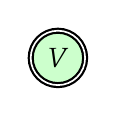
\begin{tikzpicture}[scale=1.5]
\node[finalstate] (V) at (0,0) {$V$};
\end{tikzpicture} ahová a $A\rightarrow a$ alakú szabályokat
vezetjük.\\[2ex]

A további szabályok:

\begin{tabular}{>{$}l<{$}l}
A\rightarrow aB
&
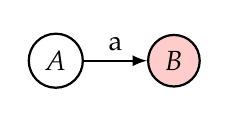
\begin{tikzpicture}[scale=1.5]
\node[state,fill=white] (A) at (0,0) {$A$};
\node[state] (B) at (1,0) {$B$};
\path[thick,->] (A) edge node[above] {a} (B);
\end{tikzpicture}
\\

A\rightarrow a
&
\begin{tikzpicture}[scale=1.5]
\node[state,fill=white] (A) at (0,0) {$A$};
\node[finalstate] (V) at (1,0) {$V$};
\path[thick,->] (A) edge node[above] {a} (B)
                ;
\end{tikzpicture}
\\

S\rightarrow \varepsilon 
&
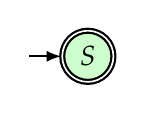
\begin{tikzpicture}[scale=1.5]
\node[finalstate] (S) at (0,0) {$S$} edge[<-,thick] (-.5,0);
\end{tikzpicture}
\\
\end{tabular}

Az átalakítás során minden nyelvtanbeli nemterminálishoz létrehozunk egy
állapotot, és a szabályok szerint megrajzoljuk a nyilakat. Ha van
$S\rightarrow \varepsilon$ szabály, akkor a kezdőállapotot egyben
végállapottá tesszük, azaz duplán karikázzuk.
\end{minipage}
} %frame vége

{\small
(Lehet-e vajon a fenti átalakításokkal ,,szabálytalan'' epszilon szabályt
létrehozni? Bizony lehet, ha a kezdő állapotból, amely végállapot is,
önmagába nyíl mutat, akkor jobboldalon is elő fog fordulni az $S$
kezdőszimbólum. Akit érdekel végiggondolhatja, hogyan lehetne
átalakítani a ,,hibás'' nyelvtant, hogy ez ne forduljon elő, de ugyanazt
a nyelvet ismerje fel. Megnyugtatásul közlöm, hogy ez megtehető a
reguláris nyelveket magában foglaló környezetfüggetlen nyelvek körében
is, és ezt a Bach-könyv ott tárgyalja.)
} %small

Az alábbi szabályok megmutatják, hogyan alakíthatunk át egy véges
automatát reguláris nyelvtanná olyan módon, hogy a reguláris nyelvtan
ugyanazt a nyelvet generálja, mint amit a véges automata felismer.
Ez az átalakítás minden esetben lehetséges, aminek az a következménye,
hogy minden véges automata reguláris nyelvet ismer fel.

\noindent
\frame{
\begin{minipage}{.98\textwidth}
\textbf{Véges automata $\rightarrow$ reguláris nyelvtan átalakítási
szabályok}

\begin{tabular}{l>{$}l<{$}}
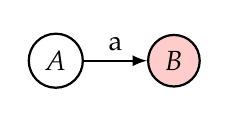
\begin{tikzpicture}[scale=1.5]
\node[state,fill=white] (A) at (0,0) {$A$};
\node[state] (B) at (1,0) {$B$};
\path[thick,->] (A) edge node[above] {a} (B);
\end{tikzpicture}
& A\rightarrow aB \\

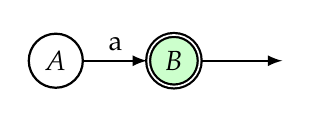
\begin{tikzpicture}[scale=1.5]
\node[state,fill=white] (A) at (0,0) {$A$};
\node[finalstate] (B) at (1,0) {$B$};
\node (C) at (2,0) {};
\path[thick,->] (A) edge node[above] {a} (B)
                (B) edge (C);
\end{tikzpicture}
& A\rightarrow aB,\quad A\rightarrow a \\

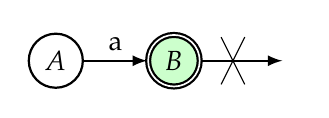
\begin{tikzpicture}[scale=1.5]
\node[state,fill=white] (A) at (0,0) {$A$};
\node[finalstate] (B) at (1,0) {$B$};
\node (C) at (2,0) {};
\path[thick,->] (A) edge node[above] {a} (B)
                (B) edge (C);
\draw (1.4,-.2) -- (1.6,+.2);
\draw (1.4,+.2) -- (1.6,-.2);
\end{tikzpicture}
& A\rightarrow a \\

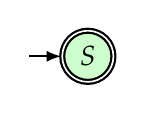
\begin{tikzpicture}[scale=1.5]
\node[finalstate] (S) at (0,0) {$S$} edge[<-,thick] (-.5,0);
\end{tikzpicture}
& S\rightarrow \varepsilon \\
\end{tabular}

Azaz ha tetszőleges állapotból nem végállapotba megyünk, vagy a
végállapotból nem vezet ki nyíl, akkor egyetlen szabállyal
helyettesíthetjük a nyilat, ha a végállapotból tovább vezet nyíl (akár
önmagába is) akkor viszont két szabállyal helyettesíthetem csak. Ha az
$S$ kezdőállapot végállapot is, akkor kell egy epszilon-szabály.
\end{minipage}
} %frame vége

Ha egyszer oda-vissza alakítunk, akkor nem feltétlenül ugyanazt a véges
automatát kapjuk, de vele egyenértékűt. Az automatává alakításkor csak a
$V$ lesz végállapot, és esetleg az $S$, míg kezdetben akár kettőnél több
végállapot is lehet.

A környezetfüggetlen nyelvek felismeréséhez már nem elegendő az DFA.
Ahhoz már az DFA-t ki kell egészíteni egy veremmel, egy olyan tárral,
aminek minden lépés során a tetejére rakhat egy elemet, vagy levehet
onnan egyet, és az állapotváltozásai során figyelembe veszi a verem
felső elemét is, ez a veremautomata (Push Down Automaton, PDA), amiről a
környezetfüggetlen nyelvek esetén lesz szó, mivel a veremautomaták a
környezetfüggetlen nyelvekkel van olyan kapcsolatban, mint a véges
automaták a reguláris nyelvekkel.

\begin{pelda}
Határozzuk meg, hogy az alábbi DFA felismeri-e a következő szavakat:
$\varepsilon$, 010, 0101, (10)$^5$? Vezesse le a 010 szót
konfigurációsorozattal! Írjuk le szavakkal és
halmazjelölésekkel, hogy milyen szavakat ismer fel! Mi a $A$ és $B$
állapotok jelentése?
Milyen típusú nyelv a felismert nyelv?
Honnan tudom, hogy determinisztikus ez a véges automata?

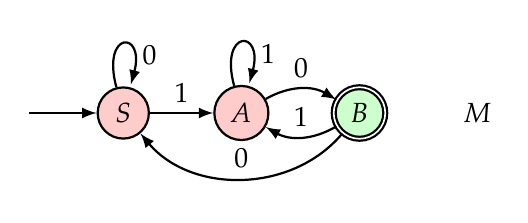
\begin{tikzpicture}[scale=1.5]
\node[state] (S) at (0,0) {$S$} edge[<-,thick] (-.8,0);
\node[state] (A) at (1,0) {$A$};
\node (cimke) at (3,0) {$M$};
\node[finalstate] (B) at (2,0) {$B$};
\path[thick,->] (S) edge node[above] {1} (A)
                     edge[loop above] node[near end,right] {0} ()
		(A) edge[loop above] node[near end,right] {1} ()
		     edge[bend left=30] node[above] {0} (B)
		(B) edge[bend left=30] node[above] {1}  (A)
		     edge[bend left=50] node[above] {0}  (S);
\end{tikzpicture}

Az üres szónál $S$-ben marad, ami nem végállapot: az üres szót nem
ismeri fel. A 010 esetén a következő állapotokon megy végig
$SSAB$. Mivel a $B$ végállapot, ezért a szót felismerte. A
0101 szó esetén ugyanazokon az állapotokon megy keresztül, csak még
visszalép a $A$-ba, ami nem végállapot, tehát a szót nem ismeri fel.
$(10)^5=1010101010$ esetén az első 1-esnél átjut $A$-ba majd $A$ és
$B$ között lépked oda-vissza. Végül a $B$-be jut, tehát felismeri az
automata.

A véges automatáknál a további lépések megállapításához elég a
pillanatnyi állapot és a bemenő szó maradék része, tehát egy
konfiguráció azt tartalmazza.
A 010 levelezése konfigurációsorozattal:
\[(S, 010) \mapsto (S, 10) \mapsto (A, 0) \mapsto (B, \varepsilon)\]
A 0101 levelezése konfigurációsorozattal:
\[(S, 0101) \mapsto (S, 101) \mapsto (A, 01) \mapsto (B, 1) \mapsto (A, \varepsilon)\]
Ha a levezetés végén elfogy a szó, és elfogadó állapotba kerülök, akkor
a szót felismerte a DFA, az automata által elfogadott nyelvhez
tartozik, ha nincs ilyen levezetés, akkor nem. Ha a fenti automatát M-el
jelöljük, akkor halmazjelölésekkel: \[010 \in {\cal L} (M), \quad 0101
\notin {\cal L} (M), \quad \{010, (10)^5, 1110\} \subset {\cal L} (M).\]

A $A$ állapotba kerül az automata bárhonnan, ha 1-est olvas. Tehát $A$
jelentése az, hogy utoljára 1-es volt a szóban. A $B$-be csak a
$A$-ból juthat az automata, ha 0-át olvas. Tehát $B$ jelentése, hogy
a szóban utoljára 10 volt. Az automata tehát azokat a szavakat ismeri
fel, amelynek a végén 10 van, azaz halmazjelöléssel:
\[{\cal L}(G) = \{y10 \mid y \in \{0,1\}^*\}.\]

Az DFA-k pontosan a reguláris nyelveket ismerik fel, tehát ${\cal L}
(M)$ reguláris nyelv.

A determinisztikusság igazolásához ellenőrizni kell minden egyes
állapotnál, hogy egyféle szimbólum hatására csak egyfelé tudok-e
továbbmenni. Jelen esetben nincs egyetlen olyan állapot sem, amelyből
két 1-es cimkéjű, vagy két 0-ás cimkéjű nyíl vezetne ki, tehát tényleg
DFA.
\end{pelda}


\subsection{Műveletek nyelvekkel}

Ismerni kell a Bach-könyv 2.5. fejezetében szereplő műveleteket:
komplemens, unió, metszet, konkatenált, hatvány, tranzitív lezárt.

\begin{itemize}
    \item Nyelvek konkatenációja: ${\cal L}_1{\cal L}_2 =
        \{xy \mid x \in {\cal L}_1,\: y \in {\cal L}_2\}$
    \item Nyelvek hatványa:  ${\cal L}^0=\{\varepsilon\},\quad
        {\cal L}^1={\cal L},\quad
        {\cal L}^2= {\cal L}{\cal L},\quad
        {\cal L}^n={\cal L}^{n-1}{\cal L}$ 
    \item Nyelvek tranzitív lezártja:  ${\cal L}^*={\cal L}^0 \cup{\cal
        L}^1 \cup{\cal L}^2 \cup{\cal L}^3 \dots$ 
\end{itemize}

Milyen nyelvek kapunk, ha ezekben a műveletekben reguláris nyelvek a
kiinduló nyelvek?

Hogyan igazoljuk ezt komplemensképzésre?

Példák. Legyen
${\cal L}_1 = \{01, 0, 101, \varepsilon \}$,\quad
      ${\cal L}_2 = \{y0y^{-1} \mid y\in \{0; 1\}^*\}$
      ekkor:
\begin{itemize}
\item ${\cal L}_1 \cap {\cal L}_2 = \{101\}$
\item $01'01010 \in {\cal L}_1{\cal L}_2$ \quad az ' csak a határt jelöli
\item $01'0'01'01'0 \in {\cal L}_1^5$
\item $01'101'01'0 \in {\cal L}_1^*$
\end{itemize}
\subsection{Reguláris kifejezések}
A reguláris kifejezéseket és reguláris halmazokat rokon értelmű szóként
használjuk. A Bach-könyv 2.6. fejezete az utóbbit, mi az előbbit
használjuk és kitérünk gyakorlati használatukra is.

Az elméleti és a gyakorlati jelölés némileg eltér egymástól, és az
utóbbi jelentősen bővebb.

A legfontosabb eltérés a jelölésben, hogy az elméletben (pl. a könyvben)
+ jelet használnak ahol a gyakorlatban függőleges vonalat ($\mid$).

Gyakorlati alkalmazást nappalisokkal laborban nézzük
(linux/vim/regexp\_vim.txt) ebből a levelezős, távos hallgatóknak csak a
* | és () valamint a karakterek levédése ($\backslash$) kell.

A gyakorlati alkalmazásban is kétféle formátuma van a reguláris
kifejezéseknek, például Java Scriptben, Pythonban a csoportosítás
zárójelét, az 1 vagy több ismétlődést jelentő +-ot és az adott számú
előfordulást jelentő \verb|{3}| zárójeleket
nem kell levédeni \verb|\|-sel (backslash-sel). Ott viszont az a
nehezebb ha kerek vagy kapcsos zárójelre kell illeszteni.  Olyankor kell
levédeni.

\section{Feladatok a nyelvcsaládokhoz és reguláris nyelvekhez, véges
automatákhoz}

A \emph{távos, levelezős} Számítástudomány tárgyhoz ezek beadandó feladatok
voltak. Újabban teszt van, amelyhez felkészüléskor érdemes ezeket
átnézni. A tesztnél lehet, hogy papíron végig kell ilyen feladatokat
vezetni, hogy válaszolni tudjunk a tesztkérdésekre.

\begin{feladat}
Határozzuk meg, hogy az ${\cal L}(G)$ nyelvben benne
van-e: $\varepsilon$, $abb$, $aabb$? Írjuk le szavakkal és
halmazjelölésekkel, milyen szavakat tartalmaz! Soroljuk be a
Chomsky-féle hierarchiába a nyelvtant!
\[\Sigma=\{a, b\},\quad N=\{S\}\] \[P=\{S\rightarrow ab;
S\rightarrow aSb\}\]
\end{feladat}

\begin{feladat}
Határozzuk meg, hogy az ${\cal L}(G)$ nyelvben benne van-e: $01$, $111$,
$1111$? Írjuk le szavakkal milyen szavakat tartalmaz! Soroljuk be a
Chomsky-féle hierarchiába a nyelvtant!
\[\Sigma=\{0, 1\},\quad N=\{S, A\}\] \[P=\{S\rightarrow 1; S\rightarrow
1A; S\rightarrow 0S; A\rightarrow 1S; A\rightarrow 0A\}\]
\end{feladat}

\begin{feladat}
Legyen adott az alábbi nyelv:
\[G = (\Sigma=\{0, 1\},\quad N=\{S, A\},\quad P=\{S\rightarrow 1; S\rightarrow
1A; S\rightarrow 0S; A\rightarrow 1S; A\rightarrow 0A\})\]

Ha lehetséges, hozzunk létre olyan $M$ véges automatát, melyre
\[{\cal L}(G) = {\cal L}(M),\]
azaz a nyelvtan által generált nyelv és az automata által felismert
nyelv megegyezik.
\end{feladat}

\begin{feladat}
Adjunk meg olyan reguláris nyelvtant, amely pontosan azokat az 0
és 1 szimbólumokból álló szavakat generálja:
  \begin{enumerate}
    \item melyek két 0-ra kezdődnek;
    \item melyekben pontosan egy 0 van.
  \end{enumerate}
\end{feladat}

\begin{feladat}
Felismeri-e az alábbi automata a csupa egyesekből álló szavakat? Adjunk
meg három olyan szót, amit az alábbi véges determinisztikus automata
felismer! Adjuk meg, milyen szavakat ismer fel (szóban vagy
halmazjelöléssel)!\\
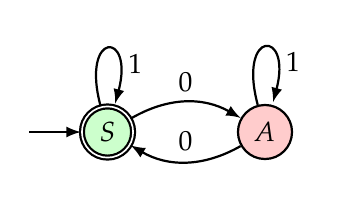
\begin{tikzpicture}[scale=2]
\node[finalstate] (S) at (0,0) {$S$} edge[<-,thick] (-.5,0);
\node[state] (A) at (1,0) {$A$};
\path[thick,->] (S) edge[bend left] node[above] {0} (A)
                     edge[loop above] node[near end,right] {1} ()
		(A) edge[loop above] node[near end,right] {1} ()
		     edge[bend left] node[above] {0} (S);
\end{tikzpicture}
\end{feladat}

\begin{feladat}
Adjunk meg DFA-t, amely az alábbi nyelvet ismeri fel, illetve
reguláris nyelvtant, amely ezt generálja: \[{\cal L}=\{x01 \mid x\in
\{0,1\}^*\}\]
\end{feladat}

\begin{feladat}
(A második típusút nem csináltunk még, az nem lesz.)
Döntsük el, hogy igazak-e az alábbi állítások. Válaszunkat
indokoljuk! (Nemleges válasz esetén általában ellenpéldával
indokolhatunk.)
  \begin{enumerate}
    \item Egy környezetfüggetlen nyelvhez létezhet olyan általános
	nyelvtan, amely azt állítja elő.
    \item A szavak konkatenációja egységelemes félcsoport.
  \end{enumerate}
\end{feladat}

\begin{feladat}
 Adjuk meg halmazleírással vagy írjuk le szavakkal milyen nyelvet
ad meg az alábbi ábrán látható véges determinisztikus automata.\\

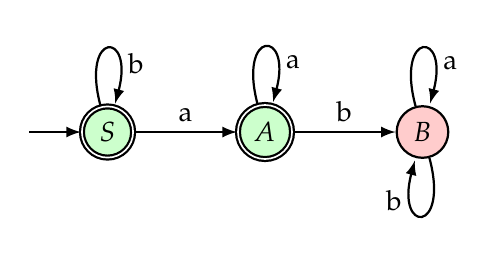
\begin{tikzpicture}[scale=2]
\node[finalstate] (S) at (0,0) {$S$} edge[<-,thick] (-.5,0);
\node[finalstate] (A) at (1,0) {$A$};
\node[state] (B) at (2,0) {$B$};
\path[thick,->] (S) edge node[above] {a} (A)
                     edge[loop above] node[near end,right] {b} ()
		(A) edge[loop above] node[near end,right] {a} ()
		     edge node[above] {b} (B)
		(B) edge[loop above] node[near end,right] {a}  ()
		     edge[loop below] node[near end, left] {b}  ();
\end{tikzpicture}
\end{feladat}

\begin{feladat}
 Hozzunk létre (lehetőleg reguláris) nyelvtant ahhoz a nyelvhez, melyet
az alábbi véges determinisztikus automata ismer fel.\\

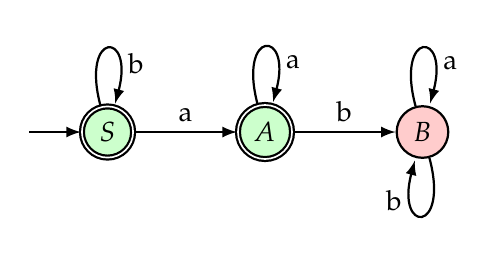
\begin{tikzpicture}[scale=2]
\node[finalstate] (S) at (0,0) {$S$} edge[<-,thick] (-.5,0);
\node[finalstate] (A) at (1,0) {$A$};
\node[state] (B) at (2,0) {$B$};
\path[thick,->] (S) edge node[above] {a} (A)
                     edge[loop above] node[near end,right] {b} ()
		(A) edge[loop above] node[near end,right] {a} ()
		     edge node[above] {b} (B)
		(B) edge[loop above] node[near end,right] {a}  ()
		     edge[loop below] node[near end, left] {b}  ();
\end{tikzpicture}
\end{feladat}

\begin{feladat}
(Nehezebb, ilyen nehéz nem lesz.)
 Adjuk meg halmazleírással vagy írjuk le szavakkal milyen nyelvet
ad meg az alábbi ábrán látható véges determinisztikus automata.\\

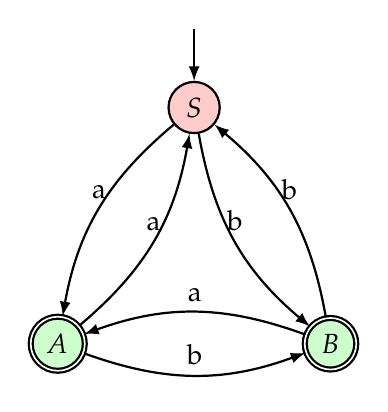
\begin{tikzpicture}[scale=2]
\node[state] (S) at (90:1) {$S$} edge[<-,thick] (90:1.5);
\node[finalstate] (A) at (210:1) {$A$};
\node[finalstate] (B) at (330:1) {$B$};
\path[thick,->] (S) edge[bend right=20] node[above] {a} (A)
                     edge[bend right=20] node[above] {b} (B)
		(A) edge[bend right=20] node[above] {a} (S)
		     edge[bend right=20] node[above] {b} (B)
		(B) edge[bend right=20] node[above] {b} (S)
		     edge[bend right=20] node[above] {a} (A);
\end{tikzpicture}
\end{feladat}

\begin{feladat}
Adjunk meg nyelvtant, amely ezt generálja:
\[{\cal L}=\{ww^{-1} \mid w\in \{0,1\}^*\}\]
\end{feladat}

\begin{feladat}
Vajon van-e olyan DFA, amely az előző feladatban szereplő nyelvet ismeri fel? 
\end{feladat}

\section{Tudnivalók és kiegészítések a környezetfüggetlen nyelvekhez}

A Bach-könyvben egy külön fejezet foglalkozik velük.

Környezetfüggetlen nyelv.

A Backus--Naur jelölés.

A nyelvtan megadásának ebben a formájában a nyíl helyett a \verb|::=|
szimbólumot használjuk, a terminális kifejezéseket idézőjelek határolják a
nemterminális szimbólumok azok, amelyeket nem idézőjelek határolnak, és egybe
írottak (az esetleges szóközt aláhúzással helyettesítik). Programozási
nyelvek megadásánál ezt szokták használni.

\begin{leftbar}
\small
\textbf{Kiegészítő anyag.}
Az alábbi túlmegy a törzsanyagon, és nem fogom kérdezni, de remélem azért lesz
aki elolvassa és hasznosnak találja.

\url{http://docs.python.org/library/string.html#formatstrings} Az itt
találhatóak szerint a Pythonban egy érték kiírási formája a következő lehet egy
sztring objektum format metódusa esetén:

\begin{verbatim}
format_spec ::=  [[fill]align][sign][#][0][width][,][.precision][type]
fill        ::=  <a character other than '}'>
align       ::=  "<" | ">" | "=" | "^"
sign        ::=  "+" | "-" | " "
width       ::=  integer
precision   ::=  integer
type        ::=  "b" | "c" | "d" | "e" | "E" | "f" | "F"
               | "g" | "G" | "n" | "o" | "s" | "x" | "X" | "%"
\end{verbatim}

Az első sorban látjuk, hogy minden nemterminális (például sign, type) szögletes
zárójelben (\verb+[]+) található, ami azt jelenti, hogy elhagyhatóak.
{\footnotesize Ez a jelölésmód nem csak nyelvek leírásában szerepel, hanem Unix
és Linux rendszerek esetén is így jelölik az elhagyható argumentumokat a
kézikönyvek SYNOPSIS sorában. Csak írjuk be a \texttt{man ls} parancsot.
\scriptsize A manból q-val lehet kilépni.}

Ennek megfelel például a \verb+"^ 8f"+ típusjelölés amely egy számot lebegőpontos
(type="f") alakban ír ki, középre rendezve (align=\verb+"^"+), ha nyolc
karakter szélességű helyre (width="8") két tizedesjegy pontossággal
(precision="2") úgy, hogy az előjelnek pozitív számoknál kihagy egy helyet
(sign=\verb'" "', szóköz) és a 8-as szélességből megmaradó helyet + karakterrel
tölti ki (fill="+")

A következő sorban egy Python kifejezés és az értéke látható:
\begin{verbatim}
"{0:+^ 8.2f}".format(1.2)
"+ 1.20++"
\end{verbatim}
\end{leftbar}

A Backus--Naur jelölésnek ettől eltérő formái is léteznek. {\small Elterjedt
még, hogy nem a terminális szimbólumokat teszik idézőjelbe, hanem a nem
terminális szimbólumokat teszik ,,kacsacsőrös'' zárójelek közé:
\verb+<értékadó operátor>+. Ilyen szerepel a könyv
1.3 fejezetében (Miért grammatika a grammatika -- Egy illusztratív
példa)}

\begin{pelda}
Írjuk tömörebb formában az alábbi Backus--Naur jelöléssel megadott nyelvtant,
majd alakítsuk át az formális nyelvek elméletében használt tömörebb
jelölésre. Az \verb+értékadó_kifejezés+-t tekintsük kezdőszimbólumnak.
\vspace{1ex}
\begin{verbatim}
értékadó_kifejezés ::= változó értékadó_operátor értékadó_kifejezés
értékadó_kifejezés ::= változó
változó ::= "a"
változó ::= "b"
értékadó_operátor ::= "="
értékadó_operátor ::= "+="
értékadó_operátor ::= "-="
értékadó_operátor ::= "*="
értékadó_operátor ::= "/="
\end{verbatim}


\textbf{Megoldás:}
A rövid forma:

\vspace{1ex}
\begin{verbatim}
értékadó_kifejezés ::= változó értékadó_operátor értékadó_kifejezés
                     | változó
változó ::= "a"
          | "b"
értékadó_operátor ::= "+="
                    | "-="
                    | "*="
                    | "/="
\end{verbatim}
\vspace{1ex}

Az \verb+értékadó_kifejezés+-t jelöljük $S$-sel, a többi nemterminálist az
ABC első nagybetűivel, a terminálisokat pedig az első kisbetűivel.

{\it
\begin{tabular}{|r|l|}
\hline
eredeti & új\\
\hline
értékadó\_kifejezés& S\\
változó&A\\
értékadó\_operátor&B\\
"a"&a\\
"b"&b\\
"="& c\\
"*="& d\\
"/="& e\\
"+="& f\\
"$-=$"& g\\
\hline
\end{tabular}
}

Így a fenti szabályok a következővé alakulnak:

\[P=\{ S \to ABS,\: S\to A,\: A\to a \mid b,\: B\to c \mid d \mid e \mid
f \mid g \}\]

Itt felhasználtuk, hogy az $A\to a$ és $A\to b$ szabályt rövidíthetjük a
$A\to a|b$ formában. Az utoló szabálycsoport is 5 szabályt foglal
magában.

Az \ref{pl:c}.  példában megnéztük, hogyan lehet levezetni belőle az
alábbi C nyelvben érvényes értékadó kifejezést.\\
\verb!a = b *= a!
\end{pelda}


\subsection{Levezetési fa}

Bal- és jobboldali levezetés.
Levezetési fa. Szintaktikai egység.
Egyértelmű, többértelmű nyelvtan.

Egyértelmű, többértelmű nyelv. Van-e algoritmus az eldöntésére?

Nyelvtanok ekvivalenciája.
Van-e algoritmus két reguláris illetve két környezetfüggetlen nyelvtan
ekvivalenciájának megállapítására? Ha van, hogyan lehet?

Ne keverjük a nyelvet és a nyelvtant!

A Bach-könyv bizonyítja, hogy az első nyelvtan (amiben E, T, F van)
egyértelmű, a bizonyítás nem kell. Ezt a nyelvtant érdemes megjegyezni.

A Bach-könyvben példa van olyan nyelvre, ami nem egyértelmű, a példát
ismerni kell, és tudni milyen szavaihoz nincs egyértelmű levezetés
semelyik hozzá tartozó CF nyelvtanban.

Reguláris nyelv lehet-e többértelmű. Milyen alakú a levezetési fája?

A könyvben szereplő nyelvtan levezetési szabályai:
\begin{equation}
    E \rightarrow E+T \mid T,\qquad T \rightarrow T*F \mid F,
    \qquad F \rightarrow (E) \mid a
    \label{eq:expr_rules}
\end{equation}

Itt kivételesen nem S-sel jelöltük a kezdőszimbólumot, hanem az angol
kifejezése kezdőbetüjével, E-vel.

Ezt a nyelvtant a Backus-Naur jelöléssel így írhatnánk.

\vspace{1ex}
\begin{verbatim}
expression ::= expression "+" term
expression ::= term
term ::= term "*" factor
term ::= factor
factor ::= "(" expression ")"
factor ::= "a"
\end{verbatim}
\vspace{1ex}

Vagy tömörebben:

\vspace{1ex}
\begin{verbatim}
expression ::= expression "+" term
             | term

term ::= term "*" factor
       | factor

factor ::= "(" expression ")"
         | "a"
\end{verbatim}
\vspace{1ex}

Ez egyes elemek jelentése magyarul: expression=kifejezés, term=tag,
factor=szorzótényező.


\subsubsection{A kifejezés nyelvének szűrése}

A nyelvtan a következő levezetési szabályokat tartalmazza:
\[
 E\rightarrow E+T | T;\quad T\rightarrow T*F| F;\quad F\rightarrow (E)|a
\]

Az $E$ (expression) a kezdőszimbólum, és a $T$ (term) és $F$ (factor) is
nemterminálisok, a többi terminális.

A nyelvtant könnyen kiegészíthetnénk úgy, hogy a kivonás és osztás
műveletét is tartalmazza, de a további vizsgálataink ez csak
bonyolítaná.

Ebben a nyelvben nincs felesleges szimbólum. Erről meggyőződhetünk, ha a
kétféle szűrést elvégezzük. Kötelezően alulról kell kezdeni a szűrést
(bottom up), a
terminális szimbólumoktól:

\begin{eqnarray*}
    B_0 = \{+, *, (, ), a\} \\
    B_1 = \{+, *, (, ), a, F\} \\
    B_2 = \{+, *, (, ), a, F, T\} \\
    B_3 = \{+, *, (, ), a, F, T, E\} \\
\end{eqnarray*}
Mivel minden szimbólum szerepel a halmazban, tehát minden
nemterminálisból levezethető valamilyen terminálisok sorozata.
folytassuk a felülről lefelé (top down) szűréssel. Itt a
kezdőszimbólummal kezdünk, amely jelen esetben az $E$.
\begin{eqnarray*}
    T_0 = \{E\} \\
    T_1 = \{E, +, T\} \\
    T_2 = \{E, +, T, *, F\} \\
    T_3 = \{E, +, T, *, F, (, ), a\} \\
\end{eqnarray*}

Ezzel megmutattuk, hogy minden szimbólum esetén van olyan szó, amely
levezethető a kezdőszimbólumból, és az adott szimbólumot tartalmazza.

\subsubsection{Reguláris nyelv levezetési fája}

A reguláris nyelvekben kétféle szabály lehet, az utolsó lépést kivéve az
$A \to aB$ alakút használjuk, ekkor mindig megmarad egy darab
nemterminális, amely a szó legvégén található. A levezetés végén egy $A
\to a$ alakú szabály használatával tudjuk a nemterminálist eltüntetni.

Egy korábbi feladatban szerepelt az alábbi levezetési szabályokkal
megadott nyelvtan. (A nagybetűk a nemterminálisok.)

\[P=\{S\rightarrow 1; S\rightarrow 1A; S\rightarrow 0S; A\rightarrow 1S; A\rightarrow 0A\}\]

Ebben érvényes az alábbi levezetés.

\[
 S \Rightarrow 1A \Rightarrow 10A \Rightarrow 101S \Rightarrow 1011
\]

A levezetés minden lépésében a jobboldalon szereplő nemterminálist
bontjuk tovább, a levezetési fa egy jobbra lefelé növő fa lesz.

\begin{tikzpicture}[
level distance=10mm,
level 1/.style={sibling distance=20mm},
level 2/.style={sibling distance=20mm},
level 3/.style={sibling distance=20mm},
level 4/.style={sibling distance=20mm}
]

\usetikzlibrary{shapes}
\tikzstyle{circ} = [draw, shape=circle]
%\tikzstyle{r} = [draw, shape=rectangle,minimum width=10mm]
\tikzstyle{leaf} = [minimum width=10mm]
\tikzstyle{tr} = [draw,isosceles triangle, shape border rotate=90, anchor=north]

\node[circ]{S}[edge from parent]
    child {node[leaf] {1}
        edge from parent coordinate (ea);
    }
    child {node[circ]{A}
        child {node[leaf]{0}
            edge from parent coordinate (ez);
        }
        child {node[circ]{A}
            child{node[leaf]{1}
                edge from parent coordinate (S);
            }
            child{node[leaf]{1}
                edge from parent coordinate (e16);
            }
            edge from parent coordinate (e30);
        }
        edge from parent coordinate (e55);
    };
\end{tikzpicture}

Ebben a nyelvtanban minden egyes szó levezetése egyetlen sorrendben
lehetséges, ami biztosítja azt, hogy egyetlen fa tartozzon a
levezetéshez. Ez a nyelvtan és így az általa meghatározott nyelv is
egyértelmű tehát. Általában bizonyítható, hogy minden reguláris nyelvhez
található egyértelmű nyelvtan, azaz \emph{a reguláris nyelvek
egyértelműek}.

\subsubsection{Eldöntő algoritmusok}

\begin{definicio}
    \emph{Két nyelvtant ekvivalensnek} nevezünk, ha ugyanazt a nyelvet
    generálják. 
\end{definicio}

Van-e olyan algoritmus, amellyel eldönthető,
\begin{enumerate}
    \item hogy két reguláris nyelvtan ekvivalens-e?

        Igen. Mindegyikhez elkészítem a véges automatát, ha nem
        determinisztikus, akkor azzá alakítom, elkészítem a
        minimálautomatát. Ha a két nyelvtanból képzett minimálautomata
        megegyezik az állapotok jelölésétől eltekintve, akkor a két
        nyelv azonos nyelvet generál.

        Az állapotok esetén lehetséges, hogy amit az egyik esetén
        $q_1$-gyel jelöltünk, a másik esetben $q_2$-vel; ettől még a két
        automata lényegében megegyezik.

    \item  hogy két környezetfüggetlen nyelvtan ekvivalens-e?

        Nem. Nemcsak hogy eddig nem tudtunk létrehozni ilyet, de
        bizonyítható, hogy nem hozható létre ilyen algoritmus.

    \item hogy egy környezetfüggetlen nyelvtan egyértelmű-e?

        Nem. Itt is bizonyítható, hogy nem hozható létre olyan
        algoritmus, amellyel ez eldönthető.
\end{enumerate}


\subsection{Környezetfüggetlen nyelvtanok átalakítása}

Mikor felesleges terminális ill. nemterminális szimbólum?

Alulról felfelé és felülről lefelé átfésülés.
Melyiknél milyen halmazzal kezdünk? Lényeges-e a sorrend?

A Bach-könyv nyomtatott (könyvként 2001-ben kiadott) változatában a nyelvtani
szabályok egyikét elírták, a következő szabályokkal igaz, hogy a
fordított sorrendű szűrés során a $C\to b$ szabály feleslegesen
bent marad, csak az a jó, ha először szűrök alulról (a terminálisoktól)
és utána felülről (a kezdőszimbólumtól):

\[S\to a,\quad S\to B,\quad B\to BC,\quad C\to b\]

Ki kell tudni szűrni felesleges szimbólumokat egy nyelvtanból.

Rekurzív szimbólum.

Álrekurzivitás, programozási példa.

Mikor rekurzív egy nyelv? Hasznos-e vagy káros a rekurzivitás?

\vspace{2em}

\begin{definicio}
    Egy nyelvtanban egy $A$ nemterminálist rekurzívnak nevezünk, ha belőle
    kiindulva levezethető olyan szó, amelyben szintén szerepel $A$.

    \[A \Rightarrow^* \alpha A \beta,
    \qquad \alpha, \beta \in (\Sigma \cup N)^*\]
\end{definicio}

A fenti definicióban $\Rightarrow^*$ (kissé logikátlanul) azt jelöli,
hogy a jobboldal egy vagy több lépésben levezethető a baloldalból.
Logikusabb lenne a $\Rightarrow^+$ jelölés.

\begin{pelda}
Adjunk példát egy programbeli álrekurzióra és egy nyelvtanbelire.

\textbf{Megoldás:}
A Python nyelvben a \verb|def| a függvénydefiniálás utasítása, a
zárójelezés helyett a sorok behúzásával tagolja a kódot. Mi a hiba
az alábbi rekurzív függvényben?

\begin{verbatim}
def factorial(n):
    return n*factorial(n-1)
\end{verbatim}

A függvény nem tud befejeződni, mert mindig újból önmagát hívja meg.
Kell tenni bele egérutat, amikor befejeződik, és nem újból önmagát
hívja:

\begin{verbatim}
def factorial(n):
    if n == 0:
        return 1
    return n*factorial(n-1)
\end{verbatim}

Ekkor, legalábbis pozitív egészekre, helyesen működik. Az első változat
álrekurzív, a második valódi rekurzív függvény.

A fentihez hasonlóan működik a $B\to bB$ szabály, ha a $B$-től sohasem
tudok megszabadulni. Az alábbi esetben C-nél ott ez egérút, B-től
viszont nem lehet megszabadulni.
\[P=\{ S \to B,\: B\to bB ,\: S\to C,\: C\to cC,\: C\to c\}\]
\end{pelda}
\vspace{2em}
Ha hozzáadnék egy $B\to b$ szabályt, akkor igazi rekurzió lenne a $B\to
bB$ és nem lenne benne felesleges szimbólum.

Mikor nem  küszöbölhető ki mindegyik $\varepsilon$-szabály?
Milyen formában engedjük meg az $\varepsilon$-szabályt olyan nyelv nyelvtanában,
amely üres szót ($\varepsilon$) tartalmaz?
Az $\varepsilon$-szabályok kiszűrési algoritmusa nem kell.

\begin{tetel}
Egy nyelvtanban minden $\varepsilon$-szabálytól megszabadulhatunk, ha az
általa generált nyelvben nincsen benne az üres szó, azaz a kezdőszimbólum
nem enyészhet el.

Ellenkező esetben a nyelvtant átalakíthatjuk úgy, hogy egyetlen
$\varepsilon$-szabályt tartalmazzon, az $S \rightarrow \varepsilon$ szabályt,
és az $S$ kezdőszimbólum nem szerepel sehol sem a levezetési szabályok
jobboldalán.
\end{tetel}

Kiküszöbölhetőek-e az egyszeres szabályok? Milyen esetben érdemes
kiszűrni? A kiszűrés algoritmusa nem kell.

Mit jelent a jólfésült nyelvtan (proper grammar)? Minden nyelvtan
átalakítható-e ilyenné?

\begin{tetel}
Minden környezetfüggetlen nyelvtannak van jólfésült egyenértékese.
\end{tetel}

A felesleges szimbólumok kiszűrése mindenképpen hasznos, de az
$\varepsilon$-szabályok és az egyszeres szabályok kiszűrése ronthat az
áttekinthetőségen.

% Tesztben.
\begin{feladat}
    Szűrjük ki az alábbi nyelvtanból a felesleges szimbólumokat!
    Határozzuk meg a nyelvtan által generált nyelvet!

\[P=\{ S \to AC,\: A\to aA ,\: C\to c,\: S\to cC,\: C\to aB,\: B\to
bE,\: F\to b\}\]
\end{feladat}

\subsection{Környezetfüggetlen nyelvtanok normálalakjai}

Milyen alakú átalakításokat tartalmazhat a Chomsky-féle normálalak
(CNF)?
Hogyan alakíthatjuk ilyenné a nyelvtant?

Milyen alakú átalakításokat tartalmazhat a Greibach-féle normálalak
(GNF)?

Benne lehet-e az $S\rightarrow \varepsilon$ szabály a normálalakokban?

Gyakran a normálalakok kevésbé áttekinthetőek, mint az eredeti nyelvtan,
de gyakran az áttekinthető nyelvtan alapján nehezebb szintaktikai
elemzőprogramot készíteni, mint a normálalakokból. Mivel a
fordítóprogramokat a számítógép futtatja, ezért az elemezhetőség
fontosabb, mint hogy az ember számára áttekinthető-e.

Mit jelent, hogy egy szimbólum balrekurzív?

Ha egy nyelv rekurzív, meg lehet-e szüntetni a rekurzivitását?

Ha egy nyelv balrekurzív, meg lehet-e szüntetni a balrekurzivitását?

Miért kell a balrekurzivitást megszüntetni?

Lehet-e a Chomsky-féle normálalak balrekurzív? Indokoljuk!

Lehet-e a Greibach-féle normálalak balrekurzív? Indokoljuk!

\subsection{Veremautomaták}

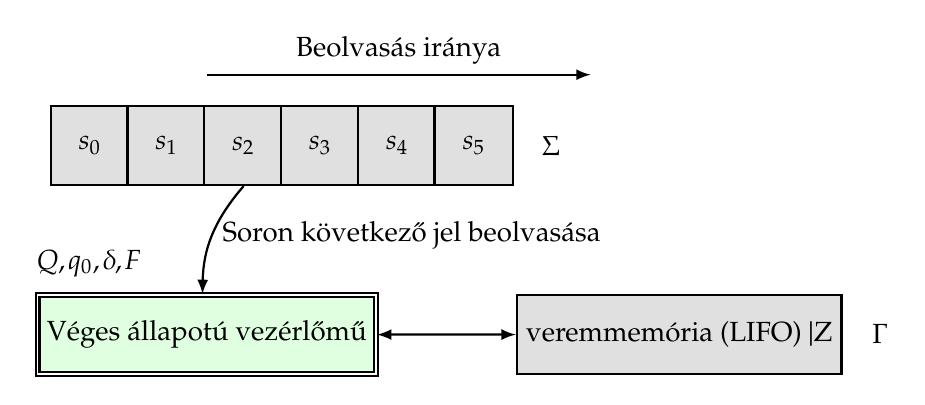
\begin{tikzpicture}[scale=1.5]
    \begin{scope}[xscale=.65,xshift=-1.52cm]
        \foreach \i in {0, 1, ..., 5}{
        \node[automat] (s\i) at (\i,0) {$s_\i$};
        }
        \node (S) at (6,0) {$\Sigma$};
    \end{scope}
\node[automat] (VM) at (4,-1.6) {veremmemória (LIFO)\:|Z};
\node (G) at (5.7,-1.6) {$\Gamma$};
\node[automat=green, double] (VA) at (0,-1.6) {Véges állapotú vezérlőmű};
\node (G) at (-1,-1) {$Q, q_0, \delta, F$};
\path[thick, ->] (s2.south) edge[bend right=20] node[right] {Soron következő jel beolvasása} (VA);
\path[thick, ->] (0,0.6) edge node[above] {Beolvasás iránya} (3.25,0.6);
\path[thick, <->] (VA) edge node[above] {} (VM);
\end{tikzpicture}

\vspace{.6em}

\begin{tabular}{|*{2}{l|}}
\hline
$\Sigma$ szalagábécé&
$q_0$ kezdőállapot ($q_0 \in Q$)
\\
$\Gamma$ veremábécé &
$Q$ állapotok
\\
$Z$ veremalja jel  ($Z \in \Gamma$)&
$F$ végállapotok  ($F \subset Q$)\\
$\delta$ mozgási szabályok&
\\
\hline
\end{tabular}

\vspace{.6em}

A veremautomata kezdetben a kezdőállapotban található, és az
,,olvasófej'' a szalag elején található, ugyanúgy, mint a véges
automatánál. A lényeges különbség abban van, hogy egy verem csatlakozik
a vezérlőműhöz, így a következő állapot attól is függhet, hogy mi van a
verem tetején. A veremautomata működésekor mi feltételezzük, hogy
minden lépésben csak a verem legtetejének a tartalmát tudjuk
megvizsgálni, és esetleg nem is vagyunk kíváncsiak erre a legfelső
elemre.

A veremben kezdetben sem üres: egy veremalja jel található benne, amit
$Z$-vel fogunk jelölni (a Bach-könyv $Z_0$-lal). Ez hasznos lesz majd,
ha meg kell vizsgálnunk, hogy leszedtük-e az összes szimbólumot, amit a
veremre raktunk. Azokat a szimbólumokat, amelyek a veremre kerülhetnek,
veremábécének nevezzük.

A következő állapot a veremautomatánál már nem csak az eredeti
állapottól és a szalagról olvasott jeltől függ\textbf{het}, hanem a
verem felső elemétől is függ\textbf{het}. A mozgási szabály ,,normál
esetben'' valahogy így néz ki a veremautomatánál:
\[\delta(q_1, b, X) = (q_2, AX)\]

Ez azt jelenti, hogyha $q_1$ állapotban van a veremautomata, a szalagon
a következő szimbólum a $b$, és a verem tetején $X$ található, akkor
átmehetünk a $q_2$ állapotba, miközben $AX$-et írunk a veremre.

A továbbiakban, amikor konfigurációsorozattal fogjuk levezetni egy szó
felismerését, a verem tartalmát egymás mellé fogjuk írni. A
verem-tartalom értelmezéséhez szükség van egy megállapodásra: mi úgy
fogjuk leírni a veremtartalmat, hogy a végén szereplő szimbólum van a
verem alján, az elején szereplő a tetején, ahogy a veremautomata
felépítéséről szóló ábrán is látható.

Tehát a fenti szabály szerint a verem tetején található szimbólum
vizsgálatához a verem tetején levő szimbólumot be kell olvasni (más
tantárgyban talán találkoztak a POP utasítással), így a fenti mozgási
szabály alkalmazásakor a verem tetejéről eltűnik az $X$, viszont
helyettel $AX$-et írok. Tehát összességében a verem tartalma annyiban
változott a két veremművelet után, hogy az eredetileg ott lévő $X$
,,fölé'' egy $A$ került.

A mozgási szabályokat majd ritkán fogjuk a fenti formában írni,
leggyakrabban állapotgráfon ábrázoljuk. A fenti átmeneti szabályt a
következő formában ábrázoljuk.

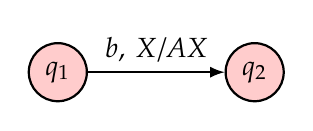
\begin{tikzpicture}[scale=2.5]
    \foreach \i in {1,2}{
    \node[state] (q\i) at (\i,0) {$q_{\i}$};
    }
    \path[thick,->] (q1) edge node[above] {$b,\:\:X/AX$} (q2);
\end{tikzpicture}

A korábbi szövegben két helyen kiemeltük a feltételes módot.
A mozgási szabályok esetén megengedjük, hogy egy mozgás során ne kelljen
mindenképpen vizsgálni a szó következő szimbólumát. Ha nem vizsgáljuk,
akkor az olvasófej sem lép tovább a következő szimbólumra. Ilyenkor a
mozgási szabályban a szimbólum helyére az üres szó jelét,
$\varepsilon$-t írjuk. Például a 
\[\delta(q_1, \varepsilon, X) = (q_2, AX)\]
mozgási szabály esetén, ha $q_1$-ben vagyok, és $X$ van a verem tetején,
akkor a szalagon következő betűtől függetlenül tovább mehetek a
következő állapotba. Ezt a fentihez hasonlóan ábrázoljuk.

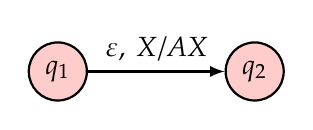
\begin{tikzpicture}[scale=2.5]
    \foreach \i in {1,2}{
    \node[state] (q\i) at (\i,0) {$q_{\i}$};
    }
    \path[thick,->] (q1) edge node[above] {$\varepsilon,\:\:X/AX$} (q2);
\end{tikzpicture}

A másik feltételes mód arra utal, hogy egy mozgási szabályban elmaradhat
a verem tetejének vizsgálata is. Ilyenkor nem is vesszük le a verem
tetejéről az ott található szimbólumot. Az alábbi első példában, az,
hogy a mozgás létrejöhet-e -- a pillanatnyi állapoton kívül -- csak a
szalagon következő szimbólumtól fog függeni, az másodikban pedig csak a
pillanatnyi állapottól.
\begin{eqnarray*}
    \delta(q_2, b, \varepsilon) &=& (q_2, B)\\
    \delta(q_1, \varepsilon, \varepsilon) &=& (q_1, AB)
\end{eqnarray*}

Fontos észrevenni, hogy a fenti szabályok esetén a $\varepsilon$ jel nem
eleme sem a veremábécének, sem a szalagábécének. A $\varepsilon$ nem egy
szimbólumot jelöl, hanem egy szót, amelynek történetesen nulla a
hosszúsága.

A mozgási szabályok tehát a függvények szokásos jelölésével leírva
következő típusúak:

\[\delta:
 Q\times (\Sigma \cup \{\varepsilon\}) \times (\Gamma \cup \{\varepsilon\})
 \longrightarrow
 Q \times \Gamma^*.
\]

A függvényérékként fellépő pár második tagja akárhány (nulla vagy több)
veremábécébeli szimbólumból állhat. Az alábbi szabályt alkalmazva
például a mozgáskor a veremről törlődik egy $X$.

\begin{equation*}
    \delta(q_2, b, X) = (q_0, \varepsilon)
\end{equation*}

A mozgási szabályok tisztázása után egy nagyon fontos lépés van hátra:
annak a tisztázása, hogy mikor mondjuk, hogy egy szalagra írt szót
felismert a veremautomata.
A veremautomatának \emph{kétféle működési módja} van, azaz
tulajdonképpen a veremautomatának kétféle definíciója, amelyekben ez a
feltétel különböző.
\begin{enumerate}
    \item A \emph{végállapottal felismerő} veremautomata (a véges
        automatákhoz hasonlóan) akkor ismeri fel a szót, ha a szó
        végigolvasásakor végállapotba kerül, vagy további lépésekkel
        végállapotba tud jutni.
    \item Az \emph{üres veremmel felismerő} veremautomata akkor ismeri
        fel a szót, ha a szó végigolvasásakor üres lesz a verem, vagy
        további lépésekkel ki tudja üríteni a vermet.
\end{enumerate}

Az üres veremmel felismerő veremautomata definiásához  nem is szükséges
végállapotokat megadni. A végállapottal felismerő veremautomatát tehát a
\begin{equation*}
    M(Q,\: q_0,\: \Sigma,\: \Gamma,\: \delta,\: F)
\end{equation*}
hatos határozza meg, az üres veremmel felismerő veremautomatát pedig az
\begin{equation*}
    M(Q,\: q_0,\: \Sigma,\: \Gamma,\: \delta)
\end{equation*}

Azt, hogy az egyik automata sem nagyobb tudású, az alábbi tétel mondja
ki.

\begin{tetel}
    Egy nyelvhez akkor és csakis akkor létezik olyan veremautomata amely
    azt végállapottal ismeri fel, ha létezik olyan veremautomata amely
    üres veremmel ismeri fel.
\end{tetel}

Ez a tétel teszi lehetővé, hogy a következő tételben (ami a
környezetfüggetlen nyelvek és a veremautomaták közötti hasonló
kapcsolatról szól, mint ami a reguláris nyelvek és a véges automaták
között van) ne kelljen pontosítani, hogy a veremautomata melyik működési
módjáról beszélünk.

\begin{tetel}
    Egy $\cal L$ nyelvet pontosan akkor ismer fel (legalább) egy
    veremautomata, ha $\cal L$ környezetfüggetlen nyelv.
\end{tetel}

A fenti két tételt mi nem bizonyítjuk. Ha valakit érdekel, a
Bach-könyvben megtalálja.

Korábban volt szó róla, hogy a véges automaták működését
konfigurációsorozattal lehet leírni. A konfiguráció tartalmazza az
összes tudást, ami ahhoz kell, hogy az automata további működése
meghatározható legyen.  A véges automatánál elegendő volt a pillanatnyi
állapot és a szalagon levő szó még nem olvasott részének ismerete. A
veremautomatánál egy harmadik dolgot, a verem teljes tartalmát is
ismerni kell. A konfigurációsorozattal történő levezetésre egy alábbi
példában és a Bach-könyvben is találhatunk példát.

\subsubsection{A kérdések, amikre tudni kell válaszolni}

Mikor mondjuk, hogy egy végállapottal felismerő veremautomata
felismert egy szót?

Mikor mondjuk, hogy egy üres veremmel felismerő veremautomata
felismert egy szót?

Miket kell megadni az egyik illetve másik megadásához?

Bővebb-e az egyik által felismert nyelvek halmaza, mint a másik által
felismerté?

Több nyelvet lehet-e felismertetni, ha nem csak a legfelső veremértéket
tudja olvasni az automata?

Melyik milyen nyelvosztályt ismer fel? (Igazolni nem kell.)

%Mikor determinisztikus egy veremautomata?

Ismerni kell az általunk órán használt gráfos megjelenítést.
A $\delta$ mozgási szabályokkal megadott alakot át kell tudni
alakítani gráffá, és viszont.

Egy szó felismerését konfigurációsorozattal meg kell tudni adni.
(Bach-könyv elektronikus változat 107. oldal.)

A verem alja szimbólumnak én a továbbiakban a $Z$-t használom $Z_0$ helyett,
igazodva a JFLAP-hez.

\begin{pelda}
Alakítsuk át az alábbi mozgási szabályokat + végállapotokat állapotgráffá!

\begin{align*}
%\delta(q_0, \varepsilon, Z) &= (q_0, \varepsilon)&
\delta(q_0, a, Z) &= (q_1, XZ)\\
\delta(q_1, a, X) &= (q_1, XX)&
\delta(q_1, b, X) &= (q_2, \varepsilon)\\
\delta(q_2, b, X) &= (q_2, \varepsilon)&
\delta(q_2, \varepsilon, Z) &= (q_0, \varepsilon)\\
F &= \{q_0\}&&\\
\end{align*}

Vezessük le konfigurációsorozattal az $aabbb$, 
$aab$, $ab$ szavakat, ha lehet. Ha nem lehet, vezessük le addig, amíg el
nem akad a levezetés.

Határozzuk meg, hogy determinisztikus-e az automata!

Milyen nyelvet fog felismerni?

\textbf{Megoldás:}

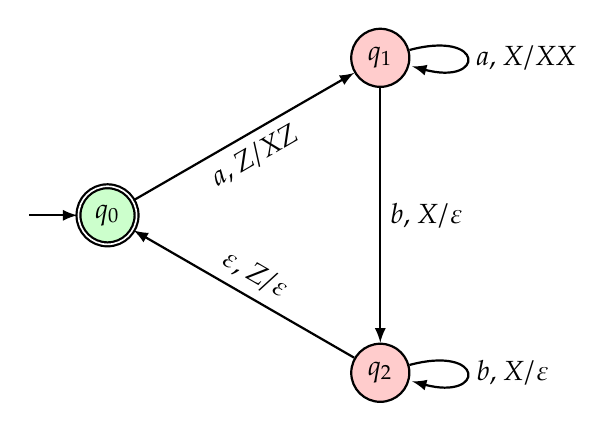
\begin{tikzpicture}[scale=2]
\node[finalstate] (S) at (0,0) {$q_0$} edge[<-,thick] (-.5,0);
\node[state] (A) at (30:2) {$q_1$};
\node[state] (B) at (-30:2) {$q_2$};
\path[thick,->] (S) edge[left=30] node[below,rotate=30] {$a,\:Z/XZ$} (A)
                 %    edge[loop above] node[above] {$\varepsilon,\:Z/\varepsilon$} ()
                (A) edge node[right] {$b,\:X/\varepsilon$} (B)
                    edge[loop right] node[right] {$a,\:X/XX$} ()
                (B) edge node[above,rotate=-30]
                {$\varepsilon,\:Z/\varepsilon$} (S)
                     edge[loop right] node[right] {$b,\:X/\varepsilon$} ();
\end{tikzpicture}

\begin{gather*}
(aabbb, q_0, Z) \to (abbb,q_1,XZ) \to (bbb,q_1,XXZ)\to\\
(bb,q_2,XZ) \to (b,q_2,Z) \not \to
\end{gather*}
Nem tudjuk végigolvasni az $aabbb$ szót, mert az utolsó szituációra nincs
szabály, amivel továbbmehetnénk. Az $aabbb$ szó tehát nem szava a fenti
veremautomata által generált nyelvnek.
\[aabbb \notin {\cal L} (M)\]

\begin{gather*}
(aab, q_0, Z) \to (ab,q_1,XZ) \to (b,q_1,XXZ)\to
(\varepsilon,q_2,XZ)
\end{gather*}

Sikerült végigolvasni a szót, de nem végállapotba jutottam, és nem is
tudok átmenni a végállapotba, mert ahhoz a verem tetején $Z$-nek kellene
lennie. Tehát $aab$ sem eleme az automata által generált nyelvnek.

\begin{gather*}
(ab, q_0, Z) \to (b,q_1,XZ) \to (\varepsilon,q_2,Z) \to
(\varepsilon,q_0,\varepsilon) 
\end{gather*}

Sikerült végigolvasni a szót, és végigolvasás után lehetőség van arra,
hogy a végállapotba átmenjünk. Tehát az automata elfogadta az $ab$ szót.
\[ab \in {\cal L} (M)\]

Az automata determinisztikus. Bár a végén $\varepsilon$ hatására megy át
$q_0$-ba, de $q_2$-ből arra a helyzetre, ha a verem tetején $Z$ van,
csak ez az egyetlen átmenet lehetséges. A véges automatáknál egy
$\varepsilon$-szabály mindig nemdeterminizmust okoz, itt a verem tetejét
is figyelni kell. A többi állapotnál pedig a kimenő
nyilakon szereplő szalagábécé-beli szimbólumok különböznek.

A fenti automata végállapotban marad, ha üres szavunk ($\varepsilon$) volt
a szó. Máskülönben csak akkor tud elindulni, ha a-val kezdődik.
Ilyenkor minden a-nál rak a veremre egy X-et. Ha b jön ezután, akkor
átmegy a $q_2$ állapotba és onnantól b szimbólumok hatására leszedegeti az
X-eket. Csak akkor tud a végén a $q_0$ végállapotba átmenni, ha az
összes X-et leszedte. Mivel ilyenkor a veramalja jel eltűnik, a
veremautomata működése nem tud folytatódni. Tehát az automata az alábbi
nyelvet fogadja el:
\[G = \{a^ib^i  \mid i \ge 0\}=\{\varepsilon, ab, aabb, aaabbb, \ldots\}\]
\end{pelda}


\subsection{Feladatok a környezetfüggetlen nyelvekhez és veremautomatákhoz}

\begin{feladat}%{51}
\[
S\rightarrow AB;\:\:
C\rightarrow aE;\:\:
A\rightarrow aA;\:\:
B\rightarrow b;\:\:
A\rightarrow a;\:\:
S\rightarrow bB;\:\:
MiK\rightarrow ULaS;\:\:
B\rightarrow bC;\:\:
E\rightarrow aC
\]

Szűrje ki a tanult módszerrel a felesleges szimbólumokat, és írja le a
megmaradt levezetési szabályokat! (A szűrés követhető legyen a papíron.)

Szűrés után az alábbi szimbólumok bizonyultak feleslegesnek:\\[1ex]
$F=\left\{\rule{0pt}{1.2em}\hspace{.7\linewidth}\right\}$.

Vezesse le lépésenként a \verb+aaaab+ szót, és rajzolja le a levezetési fáját!

\vspace{2em}
\begin{megoldas}
A Mikulásos általános, az $S\rightarrow AB$ környezetfüggetlen, a többi reguláris.

$B=\{a,b,A,B,S\}$.
Alulról szűrés után, és a legvégén is a következőek maradnak meg:
\[
S\rightarrow AB;\:\:
A\rightarrow aA;\:\:
B\rightarrow b;\:\:
A\rightarrow a;\:\:
S\rightarrow bB;\:\:
\]

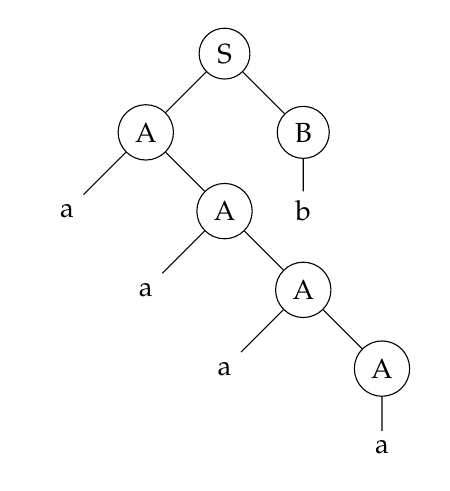
\begin{tikzpicture}[
level distance=10mm,
level 1/.style={sibling distance=20mm},
level 2/.style={sibling distance=20mm},
level 3/.style={sibling distance=20mm},
level 4/.style={sibling distance=20mm}
]

\usetikzlibrary{shapes}
\tikzstyle{circ} = [draw, shape=circle]
\tikzstyle{leaf} = [minimum width=10mm]

\node[circ]{S}[edge from parent]
    child {node[circ] {A}
        child {node[leaf]{a}
            edge from parent coordinate (l1);
        }
        child {node[circ]{A}
            child{node[leaf]{a}
                edge from parent coordinate (l2);
            }
            child{node[circ]{A}
                child{node[leaf]{a}
                    edge from parent coordinate (l3);}
                child{node[circ]{A}
                    child{node[leaf]{a}
                        edge from parent coordinate (l4);}
                    edge from parent coordinate (A4);}
                edge from parent coordinate (A3);
            }
            edge from parent coordinate (A2);
        }
        edge from parent coordinate (A);
    }
    child {node[circ]{B}
        child {node[leaf]{b}
            edge from parent coordinate (b);
        }
        edge from parent coordinate (C);
    };
\end{tikzpicture}

\end{megoldas}
\end{feladat}


\begin{feladat}{}
Határozzuk meg, hogy az alábbi automata felismeri-e üres veremmel az
\verb|abbcbba| illetve \verb+abcab+ szavakat!
Ha igen vezessük le konfigurációsorozattal!

Melyik nyelvet ismeri fel?

Adjuk meg a $\delta$  mozgásszabályokat, a $Q$ állapothalmazt, az $F$
végállapot-halmazt, az elemzendő nyelv $\Sigma$ ábécéjét, a $\Gamma$ veremábécét.

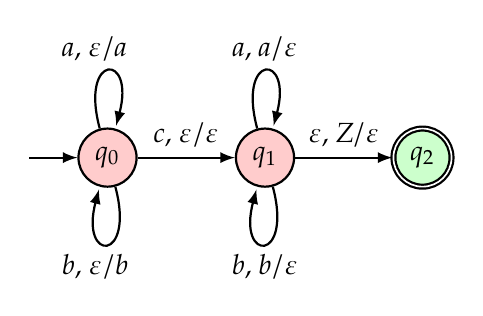
\begin{tikzpicture}[scale=2]
\node[state] (q0) at (1,0) {$q_0$} edge[<-,thick] (.5,0);
\node[state] (q1) at (2,0) {$q_1$};
\node[finalstate] (q2) at (3,0) {$q_2$};
\path[thick,->]
        (q0) edge node[above] {$c,\:\varepsilon/\varepsilon$} (q1)
            edge[loop above] node[above] {\parbox{7ex}{$a,\:\varepsilon/a$}} ()
            edge[loop below] node[below] {\parbox{7ex}{$b,\:\varepsilon/b$}} ()
        (q1) edge node[above] {$\varepsilon,\:Z/\varepsilon$} (q2)
            edge[loop above] node[above]
                {$a,\:a/\varepsilon$} ()
            edge[loop below] node[below]
                {$b,\:b/\varepsilon$} ()
        ;
\end{tikzpicture}
\end{feladat}

(Mi megengedjük, hogy a verem tetejének olvasása nélkül mehessen tovább
új állapotba. Bach Iván könyvében lévő veremautomata-változat minden
lépésben kiolvassa a verem tartalmát, legfeljebb visszaírja azt. Az
alábbi példában is ilyen szerepel. Ez az eltérés ugyanúgy nem
befojásolja a veremautomatával felismerhető nyelvek halmazát, mint ahogy
az sem, hogy üres veremmel vagy végállapottal felismerő automatát
használok-e. Érdemes lehet kitalálni, hogyan lehet csökkenteni eggyel a
szükséges állapotok számát, és jelentősen a szükséges mozgásszabályok
számát, ha kihasználjuk, hogy nem muszáj kiolvasni a veremtartalmat.)

\begin{feladat}%{33}
Az alábbi ábrán egy veremautomata állapotdiagrammja látható.

\tikzset{
  >=latex,
  state/.style ={thick,circle,draw},
  finalstate/.style ={state,double}
}
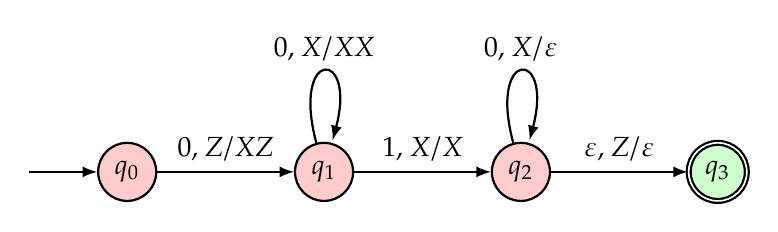
\begin{tikzpicture}[scale=2.5]
\node[state] (q0) at (0,0) {$q_0$} edge[<-,thick] (-.5,0);
\node[state] (q1) at (1,0) {$q_1$};
\node[state] (q2) at (2,0) {$q_2$};
\node[finalstate] (q3) at (3,0) {$q_3$};
\path[thick,->] (q0) edge node[above] {$0,\:Z/XZ$} (q1)
        (q1) edge node[above] {$1,\:X/X$} (q2)
            edge[loop above] node[above] {$0,\:X/XX$} ()
        (q2) edge node[above] {$\varepsilon,\:Z/\varepsilon$} (q3)
            edge[loop above] node[above] {$0,\:X/\varepsilon$} ()
        ;
\end{tikzpicture}

Vezessük le konfigurációsorozattal (amíg lehet), hogy a 00101 szót
végállapottal felismeri-e! Indokoljuk, miért vagy miért nem!

Az automata állapothalmaza $Q=$~\spacer[.4\linewidth],\\
a végállapot-halmaza $F=$~\spacer[.5\linewidth],\\
az elemzendő nyelv ábécéje $\Sigma=$~\spacer,\\
a veremábécéje $\Gamma=$~\spacer.
Két (teszőlegesen választott) $\delta$ mozgásszabálya\\ \spacer[.95\linewidth].

Határozzuk meg, hogy az alábbi automata felismeri-e végállapottal az
$\varepsilon$, 0001000 illetve 01 szavakat!

Melyik nyelvet ismeri fel?

\begin{megoldas}
A 00101, a $\varepsilon$ és a 01 szavakat nem ismeri fel, a 0001000 szót
igen.

A $\{0^i10^i \mid i>0\}$ nyelvet ismeri fel ez a veremautomata.
\end{megoldas}
\end{feladat}

\begin{feladat}{}
Határozzuk meg, hogy az alábbi automata felismeri-e végállapottal az
\verb|abba| illetve \verb+aaa+ szavakat!
Ha igen vezessük le konfigurációsorozattal!

Melyik nyelvet ismeri fel?

Adjuk meg a $\delta$  mozgásszabályokat, a $Q$ állapothalmazt, az $F$
végállapot-halmazt, az elemzendő nyelv $\Sigma$ ábécéjét, a $\Gamma$ veremábécét.

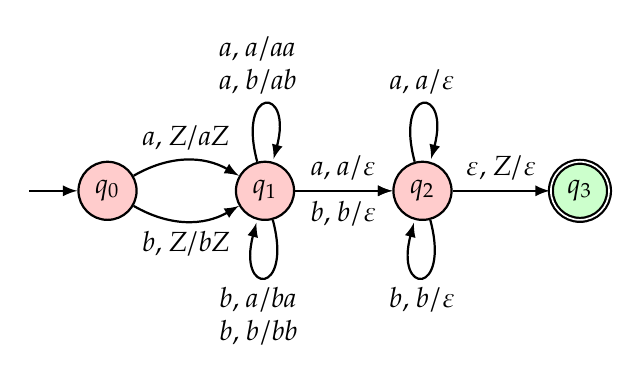
\begin{tikzpicture}[scale=2]
\node[state] (q0) at (0,0) {$q_0$} edge[<-,thick] (-.5,0);
\node[state] (q1) at (1,0) {$q_1$};
\node[state] (q2) at (2,0) {$q_2$};
\node[finalstate] (q3) at (3,0) {$q_3$};
\path[thick,->] (q0) edge[bend left=30] node[above] {$a,\:Z/aZ$} (q1)
                     edge[bend right=30] node[below] {$b,\:Z/bZ$} (q1)
        (q1) edge node[above] {$a,\:a/\varepsilon$} (q2)
             edge node[below] {$b,\:b/\varepsilon$} (q2)
            edge[loop above] node[above] {\parbox{7ex}{$a,\:a/aa$\\$a,\:b/ab$}} ()
            edge[loop below] node[below] {\parbox{7ex}{$b,\:a/ba$\\$b,\:b/bb$}} ()
        (q2) edge node[above] {$\varepsilon,\:Z/\varepsilon$} (q3)
            edge[loop above] node[above]
{$a,\:a/\varepsilon$} ()
            edge[loop below] node[below]
{$b,\:b/\varepsilon$} ()
        ;
\end{tikzpicture}
\end{feladat}

\begin{feladat}{}
  Adjon meg egy automatát, amely a szabályos zárójelezések nyelvét
  ismeri fel üres veremmel!
  \[\{ (), (()), ()(), ((())), (()()), (((()))), (()()()), ((())()),\: \dots \}\]
\end{feladat}

Figyelem! Ez nem az órán említett $\{(^i)^i \mid i>0\}$ nyelv.

\begin{feladat}
Adjunk példát az alábbi nyelvtanból álrekurzív nemterminálisra.

Az alábbi nyelvtanból csak azokat a szabályokat hagyjuk meg, amelyek nem
tartalmaznak felesleges szimbólumokat.
\[ S\to b,\quad  S\to B,\quad  S\to BC,\quad  C\to cC,\quad  B\to Bb,\quad  B\to b,\quad  C\to DC,\quad  D\to d\]

A keletkezett nyelvtanból határozzuk meg az általa generált nyelv ábécéjét, és a generált nyelvet.
\end{feladat}

\paragraph{Végeredmény}
A $C$ rekurzív (két szabály szerint is: $C\to cC,\quad  C\to DC$), ha
$C$ egyszer belekerül a levezetésbe, akkor soha nem tudunk tőle
megszabadulni, tehát álrekurzív.

Az megmaradó levezetési szabályok:
\[ S\to b,\quad  S\to B,\quad  B\to Bb,\quad  B\to b\]

A generált nyelv ábécéje $\Sigma=\{b\}$. A generált nyelv:
\[{\cal L} = \{b^i \mid i>0\}=\{b, bb, bbb, bbbb, \ldots\}\]

\begin{feladat}{}
  Hozzuk Chomsky-féle normálformára a következő nyelvtant!
  Van-e balrekurzió az eredeti, illetve a kapott nyelvtanban?
  Ha igen, hol?
\[
S\rightarrow SaSb;\qquad
S\rightarrow ab;
\]

\begin{megoldas}
  Az első átalakítás után:
\[
S\rightarrow S\hat AS\hat B;\quad
S\rightarrow \hat A\hat B;\quad
\hat A\rightarrow a ;\quad
\hat B\rightarrow b
\]
  Miután az első szabályt ,,felszeleteltük'':
\[
S\rightarrow SS_1;\quad
S_1\rightarrow \hat AS_2;\quad
S_2\rightarrow S\hat B;\quad
S\rightarrow \hat A\hat B;\quad
\hat A\rightarrow a ;\quad
\hat B\rightarrow b
\]
Mind az eredeti nyelvtan, mind a CNF-ben levőben az első levezetési
szabályban egyetlen lépésben van balrekurzió.
\end{megoldas}
\end{feladat}

\section{Tudnivalók és kiegészítések a fordító automatákhoz}

Bach könyv 4. fejezetében van szó róla.

Véges fordító (Mealy-automata változat):\\
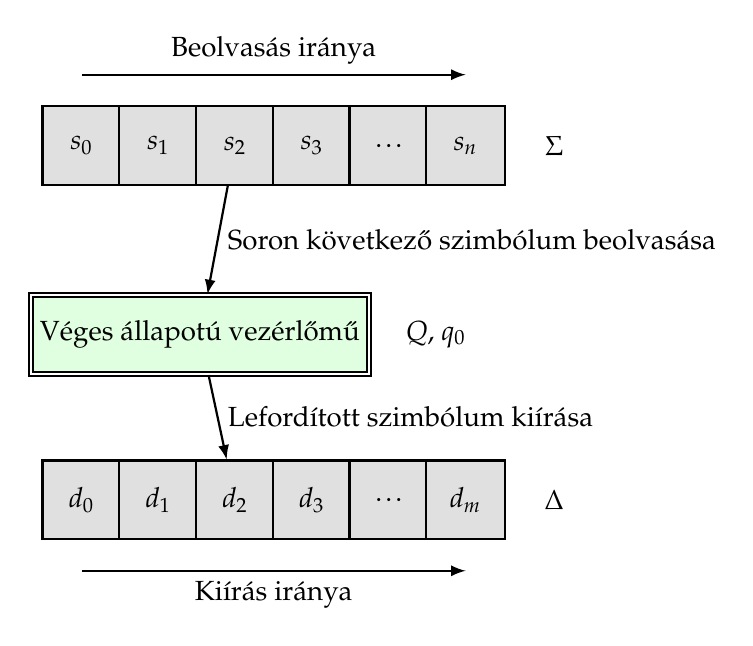
\begin{tikzpicture}[scale=1.5]
\node[automat] (s0) at (0,0) {$s_0$};
\node[automat] (s1) at (0.65,0) {$s_1$};
\node[automat] (s2) at (1.3,0) {$s_2$};
\node[automat] (s3) at (1.95,0) {$s_3$};
\node[automat] (s4) at (2.6,0) {$\ldots$};
\node[automat] (s5) at (3.25,0) {$s_n$};
\node (S) at (4,0) {$\Sigma$};
\node[automat] (q0) at (0,-3) {$d_0$};
\node[automat] (q1) at (0.65,-3) {$d_1$};
\node[automat] (q2) at (1.3,-3) {$d_2$};
\node[automat] (q3) at (1.95,-3) {$d_3$};
\node[automat] (q4) at (2.6,-3) {$\ldots$};
\node[automat] (q5) at (3.25,-3) {$d_m$};
\node (D) at (4,-3) {$\Delta$};
\node[automat=green, double] (VA) at (1,-1.6) {Véges állapotú vezérlőmű};
\node (D) at (3,-1.6) {$Q,\: q_0$};
\path[thick, ->] (s2) edge node[right] {Soron következő szimbólum beolvasása} (VA);
\path[thick, ->] (0,0.6) edge node[above] {Beolvasás iránya} (3.25,0.6);
\path[thick, ->] (VA) edge node[right] {Lefordított szimbólum kiírása} (q2);
\path[thick, ->] (0,-3.6) edge node[below] {Kiírás iránya} (3.25,-3.6);
\end{tikzpicture}

A véges fordítónak kétféle változata van. A Bach-könyv azzal
foglalkozik, amikor az átmenetek során történik a szalagra írás. Ezt a
szakirodalom Mealy-automatának nevezi. Lehet olyan véges fordítót is
készíteni, amely akkor ír a szalagra, amikor egy új állapotba kerül, ezt
a szakirodalom Moore-automatának nevezi. Belátható, hogy mindkét
fordítócsalád ugyanarra képes: tehát minden Mealy-automatához van olyan
Moore-automata, amelyek, ha azonos a bemenő szalagon lévő szó, akkor
ugyanazt írják ki a szalagra, és fordítva; minden Moore-automatához van
ilyen Mealy-automata. 

Milyen változatai vannak a véges fordítóknak? Mi a lényegi különbség a
működésükben?

Részletesen magyarázza el a Mealy-automata működését! Adjon meg egy
példát rá állapotgráffal!

\begin{feladat}
Határozza meg, mit ad vissza az alábbi ábrán szereplő automata
a \verb!baabbbaabaaabb!  szóra, azaz mire fordítja?
Mi lesz a bemeneti szalag $\Sigma$ ábécéje, és a kimeneti szalag
$\Delta$ ábécéje?

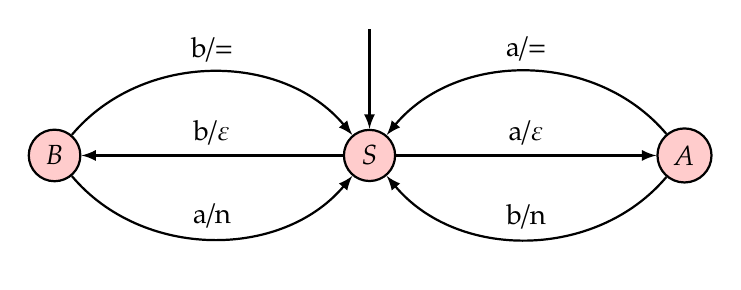
\begin{tikzpicture}[scale=4,>=latex]
\node[state] (S) at (0,0) {$S$} edge[<-,thick] (0,+.4);
\node[state] (A) at (1,0) {$A$};
\node[state] (B) at (-1,0) {$B$};
\path[thick,->] (S) edge node[above] {a/$\varepsilon$} (A)
                    edge node[above] {b/$\varepsilon$} (B)
                (A) edge[bend left=50] node[above] {b/n} (S)
                    edge[bend right=50] node[above] {a/=} (S)
                (B) edge[bend left=50] node[above] {b/=} (S)
                    edge[bend right=50] node[above] {a/n} (S);
\end{tikzpicture}

Adjon meg olyan szimbólum-sorozatot, amelynél a fenti automata esetén a
kimeneti szalagon a \verb+=nn==nn==+ jelenik meg. Egyértelmű-e ez a
szimbólum-sorozat? Ha nem, adjon meg még egyet!
\end{feladat}

A véges fordítók egy bemeneti nyelvhez egy kimeneti nyelvet rendelnek.
Azaz, ha a bemeneti nyelv minden szavára lefuttatjuk az automatát,
akkor a kimeneti szalagon kapott szavak halmazát nevezzük kimeneti
nyelvnek.

Mit mondhatunk a véges fordító kimeneti nyelvéről,
ha a bemeneti nyelve reguláris nyelvet, illetve környezetfüggetlen
nyelv?

A szintaxisvezérelt fordítási sémák 2014 tavaszán még nem kellenek.

Magyarázza el a veremfordító  működését!

Alább van egy példa veremfordítóra. Az első / előtt van, hogy mit olvas
a bemenő szalagról, utána, hogy mit ír ki a kimenő szalagra. A második
per előtt, hogy mit olvas a veremről (egy szimbólum vagy semmi), utána,
hogy mit ír rá (nulla vagy több szimbólum a veremábécéből).

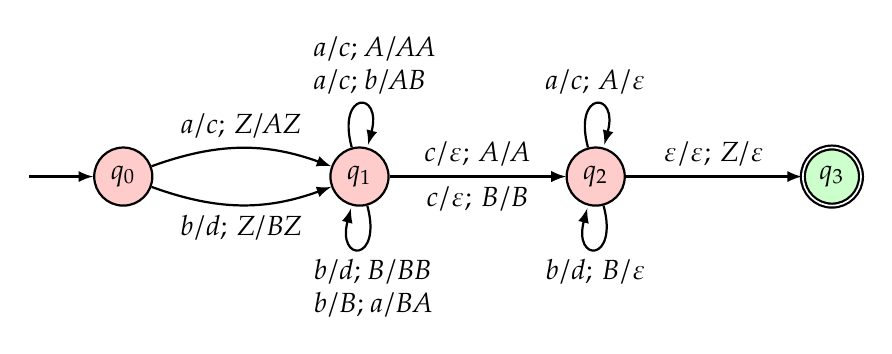
\begin{tikzpicture}[scale=1.5]
\node[state] (q0) at (0,0) {$q_0$} edge[<-,thick] (-.8,0);
\node[state] (q1) at (2,0) {$q_1$};
\node[state] (q2) at (4,0) {$q_2$};
\node[finalstate] (q3) at (6,0) {$q_3$};
\path[thick,->] (q0) edge[bend left=20] node[above] {$a/c;~Z/AZ$} (q1)
                     edge[bend right=20] node[below] {$b/d;~Z/BZ$} (q1)
                (q1) edge[loop above] node[above]
                  {\parbox{7ex}{$a/c;~A/AA$\\$a/c;~b/AB$}} ()
                     edge[loop below] node[below]
                  {\parbox{7ex}{$b/d;~B/BB$\\$b/B;~a/BA$}} ()
             edge node[above] {$c/\varepsilon;~A/A$} (q2)
             edge node[below] {$c/\varepsilon;~B/B$} (q2)
                (q2) edge[loop above] node[above] {$a/c;~A/\varepsilon$}  ()
                     edge[loop below] node[below] {$b/d;~B/\varepsilon$}  ()
             edge node[above] {$\varepsilon/\varepsilon;~Z/\varepsilon$} (q3);
\end{tikzpicture}


\newpage
\section{Tudnivalók az informatikus hallgatók Formális nyelvek
tantárgyához}
A segédletek egy része az \url{http://elearning.uni-obuda.hu} oldal
\emph{Formális nyelvek} kurzusában található.

\vspace{2ex}

Kötelező irodalom:
\begin{itemize}
\item Bach Iván: \emph{Formális nyelvek}, Typo\TeX, 2001, az Interneten
legálisan elérhető ingyenesen.
\item Az http://elearning.uni-obuda.hu oldal segédletei
\end{itemize}

Ajánlott irodalom:
\begin{itemize}
\item Roger Penrose: \emph{A császár új elméje}, Akadémiai Kiadó, 1993,
különösen Turing-géppel foglalkozó rész, de a többit is ajánlom
\item Demetrovics, Denev, Pavlov: \emph{A számítástudomány matematikai
alapjai}, Tankönyvkiadó, Budapest, 1989,
Két fejezete: 4. A formális nyelvek és automaták, 5. A Turing-gép
\item Tóth Mihály: \emph{Bevezetés a formális nyelvek és automaták
elméletébe} (Handout, 1992.)
\end{itemize}

\newpage % ++ +++ ++  ++ +++ ++  ++ +++ ++  ++ +++ ++  ++ +++ ++
%\subsection{Követelményrendszer a \emph{Formális nyelvek és gépek} tárgyhoz}
%
%(Eltérés esetén a hivatalos tantárgyi követelményrendszer a mérvadó.)
%
%A téma felbontása tantárgyi hetekre:
%\begin{enumerate}
%\item Követelményrendszer. Áttekintés: nyelvek,
%automaták vázlatosan.
%\item Nyelvek, nyelvtanok, Chomsky-féle nyelvcsaládok
%\item Nyelvek és automaták. A reguláris nyelvek és a véges
%(determinisztikus) automaták (DFA)
%\item 1. zárthelyi. Automaták vizsgálata programmal. Feladatkiosztás.
%\item Műveletek nyelvekkel. Reguláris kifejezések.
%\item Feladatbemutatás 1.
%\item Környezetfüggetlen nyelvek
%\item Veremautomaták
%\item Fordítóautomaták
%\item 2. zárthelyi. Turing-gépek fogalma
%\item Bonyolultságelmélet. Univerzális Turing-gép.
%\item Feladatbemutatás 2.
%\end{enumerate}
%
%A félév során két zárthelyi lesz, mely lehet papíron és/vagy Moodle
%tesztként. Ezek 10-10 pontosak.
%
%A félév során mindenki megcsinál egy összetettebb projektszerű
%feladatot. Ezekre két alkalommal 10 illetve 15, összesen 25 pont
%kapható.
%
%A Turing-gépekkel kapcsolatban egy Moodle-teszt lesz 5 pontért.
%
%A félév közben összesen 50 pont érhető el.
%Az aláíráshoz 25 pont elérése, és a \emph{Tanulmányi és
%vizsgaszabályzatnak} megfelelő részvételi arány szükséges. Akinek
%nincsen meg, az a két zárthelyiből javíthat (várhatóan papíron).
%
%A vizsgán két tételt húzhat a tananyag első és második feléből.
%Mindegyik tételhez egy kapcsolódó feladatot is kapnak.
%
%NSZHA1SANB 2+0+0 v 2, előkövetelmény Szoftver szigorlat (NSZSS1SANB) 
%%C-s tantervben modulok része

\subsection{2011. tavaszi beadandó feladatok, nappali info}

DFA = determinisztikus véges automata

Az alábbi feladatokat JFLAP-pel kell megoldani. Az automatához legalább
öt-öt jól választott elfogadott és elutasított szót kell kipróbálni.
Több feladathoz is kellhet, hogy a 0 is páros szám.

\begin{enumerate}
\item Készítsen olyan DFA-t, amely azokat a 0 és 1 szimbólumokból
álló nyelvet fogadják el, amelyek páratlan 1-est tartalmaznak!
%- Berencsi Gergő

\item Készítsen olyan DFA-t, amely azokat a 0 és 1 szimbólumokból
álló nyelvet fogadják el, amelyek páros 1-est tartalmaznak!
%- Kucsera Gergely

\item Készítsen olyan DFA-t, amelyek azt a nyelvet fogadják el, amelyben
tetszőleges számú \verb|a| után páros számú \verb|b| szimbólum jön!
%- Németh Norbert

\item Készítsen olyan DFA-t, amelyek azt a nyelvet fogadják el, amelyben
tetszőleges számú \verb|a| után páratlan számú \verb|b| szimbólum jön!
%- Páros Zoltán

\item Készítsen olyan DFA-t, amelyek azt a nyelvet fogadják el, amelyben
két vagy három \verb|a| után ugyanannyi \verb|b| szimbólum jön!
%- Porteleki Gábor

\item Készítsen olyan DFA-t, amelyek azt a nyelvet fogadják el, amelyben
két vagy három \verb|a| után eggyel kevesebb \verb|b| szimbólum jön!
%- Róth Bálint

\item Készítsen olyan DFA-t, amelyek azt a nyelvet fogadják el, melynek
szavaiban csak \verb|a| és \verb|b| szimbólum lehet, és csak páratlan
hosszúságú szavak.
%- Schlett Péter

\item Készítsen olyan DFA-t, amelyek olyan a és b szimbólumokból álló szavakat
fogad el, amelyek ab-re végződnek.
%- Szücs Máté

\item Készítsen olyan DFA-t, amelyek olyan a és b szimbólumokból álló szavakat
fogad el, amelyek nem ab-re végződnek.
%- Balázs András

\item Készítsen olyan DFA-t, amelyek olyan szavakat fogad el, amelyek néggyel
osztható számok bináris formái.
%- Boór Katalin

\item Készítsen olyan DFA-t, amelyek olyan szavakat fogad el, amelyek néggyel
nem osztható számok bináris formái.
%- Bőcs Gergő

\item Készítsen olyan DFA-t, amelyek olyan 0 és 1 szimbólumokból álló szavakat
fogad el, amelyben nem szerepel két 1-es egymás után.
%- Dunaszegi Péter

\item Készítsen olyan DFA-t, amelyek olyan a és b szimbólumokból álló szavakat
fogad el, amelyben van 2 egymás utáni a szimbólum.
- Imre Mária

\item Készítsen olyan DFA-t, amelyek olyan 0 és 1 szimbólumokból álló szavakat
fogad el, amelyben szerepel a 010 szimbólumsorozat.
%- Kiss Máté

\item Készítsen olyan DFA-t, amelyek olyan 0 és 1 szimbólumokból álló szavakat
fogad el, amelyben nem szerepel a 010 szimbólumsorozat.
%- László Róbert

\item Készítsen olyan DFA-t, amelyek olyan . és \verb|-| szimbólumokból álló szavakat
fogad el, amelyben szerepel a \verb|...---...| szimbólumsorozat.

\item Készítsen olyan DFA-t, amelyek olyan . és - szimbólumokból álló szavakat
fogad el, amelyben nem szerepel a \verb|...---...| szimbólumsorozat.
\end{enumerate}


%\subsection{Régebbi beadandó feladatok}
%
%Ezek a feladatok a  Formális nyelvek tantárgyhoz, az informatikus
%hallgatóknak szóltak. A villamosmérnök tárgyhoz más beadandó tartozik.
%
%Készítsünk el a LaTeX tikz csomagjával egy véges automata, egy
%veremautomata, egy véges fordító és egy veremfordító gráfját. Az első
%kettő esetén írjuk le LaTeX-ben a hozzájuk tartozó nyelvet és egy
%hozzájuk tartozó nyelvtant. Az automatáknál minimálisan 4 állapot
%kell és $\Sigma$ minimum két elemű legyen.
%
%Felhasználható ennek a dokumentumnak a forráskódja.
%
%A tikz/pgf dokumentációja:\\
%/usr/share/doc/texmf/pgf/pgfmanual.pdf.gz 
%
%\begin{tikzpicture}[scale=1.5]
%\node[state] (S) at (0,0) {$S$} edge[<-,thick] (-.8,0);
%\node[state] (A) at (1,0) {$A$};
%\node[finalstate] (B) at (2,0) {$B$};
%\path[thick,->] (S) edge node[above] {1} (A)
%                     edge[loop above] node[right] {0} ()
%		(A) edge[loop above] node[near end,right] {1} ()
%		     edge[bend left=30] node[anchor=270] {0} (B)
%		(B) edge[bend left=30] node[left] {1}  (A)
%		     edge[bend left=50] node[near end,below]
%		     {$a/A;\:X/\varepsilon$}  (S);
%\end{tikzpicture}
%
%A generált nyelv az
%\[{\cal L} = \{ a^ib^j \mid i>3, j\ge 2\}.\]

\section{Tételsor}

\begin{enumerate}
    \item Nyelvek, nyelvtanok, automaták kapcsolata. Mit jelent, hogy
        egy nyelvtan generál egy nyelvet, ill. egy automata felismer egy
        nyelvet? Milyen automaták társíthatóak a nyelvosztályokhoz
        (villamosmérnököknek csak a két legszűkebb nyelvosztályhoz)?
    \item Chomsky-féle nyelv- és nyelvtan-osztályok
    \item Véges automaták felépítése, működése, megadásuk
        állapotgráffal, és csoportosításuk (determinisztikusság,
        teljesség)
    \item Reguláris nyelvek és a véges automaták kapcsolata, egymásba
        alakítása
    \item Műveletek nyelvekkel (komplemens, unio, metszet, konkatenáció,
        tranzitív lezárt). Milyen nyelv lesz ezek eredménye a reguláris
        nyelvek esetén?
    \item Reguláris kifejezések
    \item Környezetfüggetlen nyelvtanok és nyelvek egyértelműsége; a két
        műveletet és zárójelet tartalmazó kifejezések (E, T, F
        nemterminálisokat tartalmazó) nyelvtana; levezetési fa; példa
        nem egyértelmű nyelvre
    \item Programozási nyelvek nyelvtanának megadása Backus-Naur
        normálalakban; honnan ismerhetőek fel a terminálisok,
        nemterminálisok
    \item Környezetfüggetlen nyelvtanok jólfésült nyelvtanná alakítása
    \item Környezetfüggetlen nyelvtanok normálalakjai, Chomsky-féle
        normálalakra alakítás, rekurzió, balrekurzió
    \item Veremautomaták felépítése és működése, megadása
        állapotgráffal, típusai (végállapottal ill. üres veremmel
        felismerő), levezetés konfigurációsorozattal
\end{enumerate}

\hrulefill

Csak informatikusoknak:

\begin{enumerate}
    \setcounter{enumi}{11}
    \item Milyen algoritmikusan eldönthető és eldönthetetlen problémákat
        ismerünk a formális nyelvekkel kapcsolatban?
    %\item Fordítóautomaták felépítése és működése, típusai, megadása
    %    állapotgráffal
    %\item Turing-gépek felépítése és működése, megadása
    %    állapotgráffal, típusai, ekvivalenciájuk.
\end{enumerate}


\newpage
\tableofcontents
\end{document}
